\phantomsection
\section*{Chapter 1}
\addcontentsline{toc}{section}{Chapter 1}

\subsection*{1.4}

\begin{figure}[H]
  \centering
  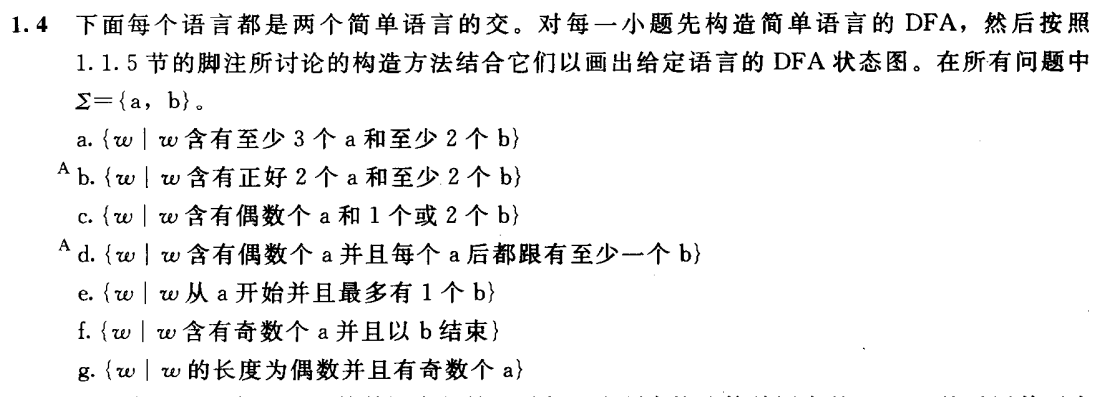
\includegraphics[width=\textwidth]{chapters/imgs/hw_1_4.png}
  \caption{}
  \label{fig:hw_1_4}
\end{figure}

% ============================================================
% 小题 a:至少 3 个 a 且至少 2 个 b
% ============================================================
\subsubsection*{(a) $\{w \mid w$ 含至少 3 个 a 和至少 2 个 b$\}$}

状态 $(i,j)$:$i$ = a 的计数(3 饱和),$j$ = b 的计数(2 饱和)。接受态 $(3, \ge 2)$。

\begin{center}
\begin{tikzpicture}[shorten >=1pt, auto, node distance=1.9cm, on grid]
    \matrix (m) [matrix of nodes,
                 nodes={state},
                 row sep=1.7cm, column sep=2.1cm] {
        $0,0$ & $0,1$ & $0,{\geq}2$ \\
        $1,0$ & $1,1$ & $1,{\geq}2$ \\
        $2,0$ & $2,1$ & $2,{\geq}2$ \\
        $3,0$ & $3,1$ & |[state, accepting]| $3,{\geq}2$ \\
    };
    % 起始箭头
    \draw[->] ([xshift=-1cm]m-1-1.west) -- (m-1-1.west);
    % 水平箭头 (b)
    \foreach \r in {1,2,3,4} {
        \draw[->] (m-\r-1) -- node {b} (m-\r-2);
        \draw[->] (m-\r-2) -- node {b} (m-\r-3);
    }
    % 垂直箭头 (a)
    \foreach \c in {1,2,3} {
        \draw[->] (m-1-\c) -- node[swap] {a} (m-2-\c);
        \draw[->] (m-2-\c) -- node[swap] {a} (m-3-\c);
        \draw[->] (m-3-\c) -- node[swap] {a} (m-4-\c);
    }
    % b 饱和自环(第 3 列)
    \foreach \r in {1,2,3,4} {
        \draw[->] (m-\r-3) edge[loop right] node {b} ();
    }
    % a 饱和自环(第 4 行)
    \foreach \c in {1,2,3} {
        \draw[->] (m-4-\c) edge[loop below] node {a} ();
    }
\end{tikzpicture}
\end{center}

% ============================================================
% 小题 b:恰好 2 个 a 且至少 2 个 b
% ============================================================
\subsubsection*{(b) $\{w \mid w$ 含正好 2 个 a 和至少 2 个 b$\}$}

第 4 行 $(\ge 3, \cdot)$ 为死状态(红色),接受态仅 $(2, \ge 2)$。

\begin{center}
\begin{tikzpicture}[shorten >=1pt, auto, node distance=1.9cm, on grid]
    \matrix (m) [matrix of nodes,
                 nodes={state},
                 row sep=1.7cm, column sep=2.1cm] {
        $0,0$ & $0,1$ & $0,{\geq}2$ \\
        $1,0$ & $1,1$ & $1,{\geq}2$ \\
        $2,0$ & $2,1$ & |[state, accepting]| $2,{\geq}2$ \\
        |[state, dead]| ${\geq}3,0$ & |[state, dead]| ${\geq}3,1$ & |[state, dead]| ${\geq}3,{\geq}2$ \\
    };
    \draw[->] ([xshift=-1cm]m-1-1.west) -- (m-1-1.west);
    \foreach \r in {1,2,3,4} {
        \draw[->] (m-\r-1) -- node {b} (m-\r-2);
        \draw[->] (m-\r-2) -- node {b} (m-\r-3);
    }
    \foreach \c in {1,2,3} {
        \draw[->] (m-1-\c) -- node[swap] {a} (m-2-\c);
        \draw[->] (m-2-\c) -- node[swap] {a} (m-3-\c);
        \draw[->] (m-3-\c) -- node[swap] {a} (m-4-\c);
    }
    \foreach \r in {1,2,3,4} {
        \draw[->] (m-\r-3) edge[loop right] node {b} ();
    }
    \foreach \c in {1,2,3} {
        \draw[->] (m-4-\c) edge[loop below] node {a} ();
    }
\end{tikzpicture}
\end{center}

% ============================================================
% 小题 c:偶数个 a 且 1 或 2 个 b
% ============================================================
\subsubsection*{(c) $\{w \mid w$ 含偶数个 a 和 1 个或 2 个 b$\}$}

行:a 奇偶(E/O);列:b 计数 0, 1, 2, $\ge 3$(死)。接受态 $(E,1)$ 和 $(E,2)$。

\begin{center}
\begin{tikzpicture}[shorten >=1pt, auto, node distance=1.9cm, on grid]
    \matrix (m) [matrix of nodes,
                 nodes={state},
                 row sep=1.8cm, column sep=2cm] {
        $E,0$ & |[state, accepting]| $E,1$ & |[state, accepting]| $E,2$ & |[state, dead]| $E,{\geq}3$ \\
        $O,0$ & $O,1$ & $O,2$ & |[state, dead]| $O,{\geq}3$ \\
    };
    \draw[->] ([xshift=-1cm]m-1-1.west) -- (m-1-1.west);
    % 水平 (b)
    \foreach \r in {1,2} {
        \draw[->] (m-\r-1) -- node {b} (m-\r-2);
        \draw[->] (m-\r-2) -- node {b} (m-\r-3);
        \draw[->] (m-\r-3) -- node {b} (m-\r-4);
    }
    % 垂直双向 (a 翻转奇偶)
    \foreach \c in {1,2,3,4} {
        \draw[->] (m-1-\c) edge[bend left=15]  node {a}       (m-2-\c);
        \draw[->] (m-2-\c) edge[bend left=15]  node {a}       (m-1-\c);
    }
    % 死状态自环
    \draw[->] (m-1-4) edge[loop right] node {a,b} ();
    \draw[->] (m-2-4) edge[loop right] node {a,b} ();
\end{tikzpicture}
\end{center}

\textit{注:死列箭头 $a$ 实际指向另一行的死态,本图已用两条双向箭头覆盖。}

% ============================================================
% 小题 d:偶数个 a 且每个 a 后跟至少一个 b
% ============================================================
\subsubsection*{(d) $\{w \mid w$ 含偶数个 a 且每个 a 后跟至少一个 b$\}$}

行:a 奇偶 E/O;列:$B_0$ (可接受)、$B_1$ (刚读 a 等 b)、$B_d$死。唯一接受 $(E, B_0)$。

\begin{center}
\begin{tikzpicture}[shorten >=1pt, auto, node distance=3cm, on grid]
    \node[state, initial, accepting]  (EB0)                    {$E,B_0$};
    \node[state]                      (OB1) [right=of EB0]     {$O,B_1$};
    \node[state, dead]                (EDd) [right=of OB1]     {$E,B_d$};
    \node[state]                      (OB0) [below=of EB0]     {$O,B_0$};
    \node[state]                      (EB1) [right=of OB0]     {$E,B_1$};
    \node[state, dead]                (ODd) [right=of EB1]     {$O,B_d$};
    \path[->]
        % (E,B0): a -> (O,B1); b 自环
        (EB0) edge [bend left=10]    node        {a} (OB1)
        (EB0) edge [loop above]      node        {b} ()
        % (O,B1): a -> (E,Bd); b -> (O,B0)
        (OB1) edge                   node        {a} (EDd)
        (OB1) edge                   node        {b} (OB0)
        % (O,B0): a -> (E,B1); b 自环
        (OB0) edge [bend left=10]    node        {a} (EB1)
        (OB0) edge [loop below]      node        {b} ()
        % (E,B1): a -> (O,Bd); b -> (E,B0)
        (EB1) edge                   node        {a} (ODd)
        (EB1) edge                   node [swap] {b} (EB0)
        % 死状态: a 翻转 E/O, b 自环
        (EDd) edge [bend left=10]    node        {a} (ODd)
        (ODd) edge [bend left=10]    node        {a} (EDd)
        (EDd) edge [loop above]      node        {b} ()
        (ODd) edge [loop below]      node        {b} ();
\end{tikzpicture}
\end{center}
\textbf{案：}

% ============================================================
% 小题 e:以 a 开头且最多 1 个 b
% ============================================================
\subsubsection*{(e) $\{w \mid w$ 从 a 开始且最多 1 个 b$\}$}

只绘从起始态可达的 6 个状态。接受态 $(S_a, 0)$ 和 $(S_a, 1)$。

\begin{center}
\begin{tikzpicture}[shorten >=1pt, auto, node distance=2.8cm, on grid]
    \node[state, initial]         (S0)                     {$S_0,0$};
    \node[state, accepting]       (Sa0) [below=of S0]      {$S_a,0$};
    \node[state, accepting]       (Sa1) [right=of Sa0]     {$S_a,1$};
    \node[state, dead]            (SaD) [right=of Sa1]     {$S_a,{\geq}2$};
    \node[state, dead]            (Sd1) [right=3cm of S0]  {$S_d,1$};
    \node[state, dead]            (SdD) [right=of Sd1]     {$S_d,{\geq}2$};

    \path[->]
        (S0)  edge                 node {a}   (Sa0)
        (S0)  edge                 node {b}   (Sd1)
        (Sa0) edge [loop left]     node {a}   ()
        (Sa0) edge                 node {b}   (Sa1)
        (Sa1) edge [loop above]    node {a}   ()
        (Sa1) edge                 node {b}   (SaD)
        (SaD) edge [loop right]    node {a,b} ()
        (Sd1) edge [loop above]    node {a}   ()
        (Sd1) edge                 node {b}   (SdD)
        (SdD) edge [loop right]    node {a,b} ();
\end{tikzpicture}
\end{center}

% ============================================================
% 小题 f:奇数个 a 且以 b 结尾
% ============================================================
\subsubsection*{(f) $\{w \mid w$ 含奇数个 a 且以 b 结束$\}$}

状态:$(\text{a 奇偶}, \text{末字符})$。起始态 $(E,a)$(空串归此类)。接受态 $(O,b)$。

\begin{center}
\begin{tikzpicture}[shorten >=1pt, auto, node distance=3cm, on grid]
    \node[state, initial]      (Ea)                  {$E,a$};
    \node[state]               (Oa) [right=of Ea]    {$O,a$};
    \node[state]               (Eb) [below=of Ea]    {$E,b$};
    \node[state, accepting]    (Ob) [right=of Eb]    {$O,b$};

    \path[->]
        (Ea) edge [bend left=15] node        {a} (Oa)
        (Oa) edge [bend left=15] node        {a} (Ea)
        (Ea) edge                node        {b} (Eb)
        (Oa) edge                node        {b} (Ob)
        (Eb) edge [bend left=15] node        {a} (Oa)
        (Ob) edge [bend left=15] node[swap]  {a} (Ea)
        (Eb) edge [loop left]    node        {b} ()
        (Ob) edge [loop right]   node        {b} ();
\end{tikzpicture}
\end{center}

% ============================================================
% 小题 g:长度为偶数且奇数个 a
% ============================================================
\subsubsection*{(g) $\{w \mid |w|$ 为偶数且 $w$ 有奇数个 a$\}$}

状态:(长度奇偶, a 奇偶)。任何字符都翻转长度;a 额外翻转 a 计数。接受态 $(L_e, A_o)$。

\begin{center}
\begin{tikzpicture}[shorten >=1pt, auto, node distance=3.5cm, on grid]
    \node[state, initial]      (EE)                  {$L_e,A_e$};
    \node[state, accepting]    (EO) [right=of EE]    {$L_e,A_o$};
    \node[state]               (OE) [below=of EE]    {$L_o,A_e$};
    \node[state]               (OO) [right=of OE]    {$L_o,A_o$};

    \path[->]
        (EE) edge [bend left=15]  node        {a} (OO)
        (OO) edge [bend left=15]  node        {a} (EE)
        (EE) edge [bend left=15]  node        {b} (OE)
        (OE) edge [bend left=15]  node        {b} (EE)
        (EO) edge [bend left=15]  node        {a} (OE)
        (OE) edge [bend left=15]  node        {a} (EO)
        (EO) edge [bend right=15] node[swap]  {b} (OO)
        (OO) edge [bend right=15] node[swap]  {b} (EO);
\end{tikzpicture}
\end{center}

\vspace{2em}
\textbf{观察:}由 $|w| = \#_a + \#_b$,$|w|$ 偶且 $\#_a$ 奇 $\Longleftrightarrow \#_b$ 亦为奇数,
所以此语言等价于 $\{w \mid \#_a, \#_b$ 均为奇数$\}$。

\paragraph{案：}“和”、“并且”等表示的是

\subsection*{1.5}

\begin{figure}[H]
  \centering
  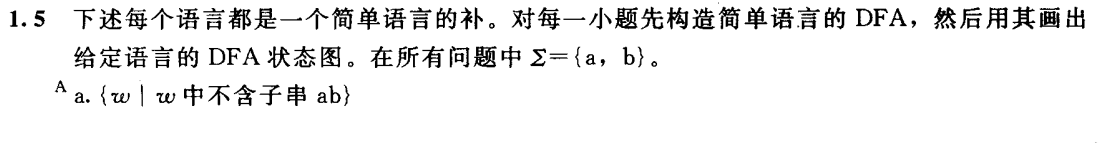
\includegraphics[width=\textwidth]{chapters/imgs/hw_1_5_p1.png}
  \caption{}
  \label{fig:hw_1_5_p1}
\end{figure}

\begin{figure}[H]
  \centering
  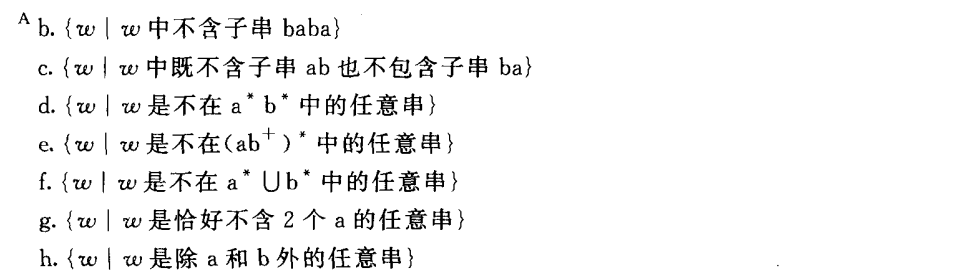
\includegraphics[width=\textwidth]{chapters/imgs/hw_1_5_p2.png}
  \caption{}
  \label{fig:hw_1_5_p2}
\end{figure}

解答：
\noindent\textbf{方法总结:}对每小题先给简单语言 $L_1$ 构造完备 DFA $M$(所有状态对所有字符都必须有转移,必要时添加死状态),然后将接受态集 $F$ 换成 $Q\setminus F$,得到识别 $\overline{L_1}$ 的 DFA。转移保持不变。

% ============================================================
% 小题 a:不含子串 ab
% ============================================================
\subsubsection*{(a) $\{w \mid w$ 中不含子串 $ab\}$}

简单语言 $L_1 = \{w \mid w$ 含子串 $ab\}$。

\vspace{0.5em}
\noindent\textbf{$L_1$ 的 DFA:}
\begin{center}
\begin{tikzpicture}[shorten >=1pt, auto, node distance=2.8cm, on grid]
    \node[state, initial]    (q0)              {$q_0$};
    \node[state]             (q1) [right=of q0] {$q_1$};
    \node[state, accepting]  (q2) [right=of q1] {$q_2$};
    \path[->]
        (q0) edge              node {a}   (q1)
        (q1) edge              node {b}   (q2)
        (q0) edge [loop above] node {b}   ()
        (q1) edge [loop above] node {a}   ()
        (q2) edge [loop above] node {a,b} ();
\end{tikzpicture}
\end{center}

\noindent\textbf{$\overline{L_1}$ 的 DFA}(接受态互换):
\begin{center}
\begin{tikzpicture}[shorten >=1pt, auto, node distance=2.8cm, on grid]
    \node[state, initial, accepting]  (q0)              {$q_0$};
    \node[state, accepting]           (q1) [right=of q0] {$q_1$};
    \node[state, dead]                (q2) [right=of q1] {$q_2$};
    \path[->]
        (q0) edge              node {a}   (q1)
        (q1) edge              node {b}   (q2)
        (q0) edge [loop above] node {b}   ()
        (q1) edge [loop above] node {a}   ()
        (q2) edge [loop above] node {a,b} ();
\end{tikzpicture}
\end{center}

% ============================================================
% 小题 b:不含子串 baba
% ============================================================
\subsubsection*{(b) $\{w \mid w$ 中不含子串 $baba\}$}

简单语言 $L_1 = \{w \mid w$ 含子串 $baba\}$。失配回退是关键:$q_3$ 读 b 退回 $q_1$(新 b 可为新匹配开头);$q_2$ 读 a 退回 $q_0$。

\noindent\textbf{$L_1$ 的 DFA:}
\begin{center}
\begin{tikzpicture}[shorten >=1pt, auto, node distance=2.6cm, on grid]
    \node[state, initial]    (q0)                   {$q_0$};
    \node[state]             (q1) [right=of q0]     {$q_1$};
    \node[state]             (q2) [right=of q1]     {$q_2$};
    \node[state]             (q3) [right=of q2]     {$q_3$};
    \node[state, accepting]  (q4) [right=of q3]     {$q_4$};
    \path[->]
        (q0) edge                  node {b}   (q1)
        (q1) edge                  node {a}   (q2)
        (q2) edge                  node {b}   (q3)
        (q3) edge                  node {a}   (q4)
        (q0) edge [loop above]     node {a}   ()
        (q1) edge [loop above]     node {b}   ()
        (q2) edge [bend left=40]   node {a}   (q0)
        (q3) edge [bend left=35]   node {b}   (q1)
        (q4) edge [loop above]     node {a,b} ();
\end{tikzpicture}
\end{center}

\noindent\textbf{$\overline{L_1}$ 的 DFA:}
\begin{center}
\begin{tikzpicture}[shorten >=1pt, auto, node distance=2.6cm, on grid]
    \node[state, initial, accepting]  (q0)                   {$q_0$};
    \node[state, accepting]           (q1) [right=of q0]     {$q_1$};
    \node[state, accepting]           (q2) [right=of q1]     {$q_2$};
    \node[state, accepting]           (q3) [right=of q2]     {$q_3$};
    \node[state, dead]                (q4) [right=of q3]     {$q_4$};
    \path[->]
        (q0) edge                  node {b}   (q1)
        (q1) edge                  node {a}   (q2)
        (q2) edge                  node {b}   (q3)
        (q3) edge                  node {a}   (q4)
        (q0) edge [loop above]     node {a}   ()
        (q1) edge [loop above]     node {b}   ()
        (q2) edge [bend left=40]   node {a}   (q0)
        (q3) edge [bend left=35]   node {b}   (q1)
        (q4) edge [loop above]     node {a,b} ();
\end{tikzpicture}
\end{center}

% ============================================================
% 小题 c:既不含 ab 也不含 ba
% ============================================================
\subsubsection*{(c) $\{w \mid w$ 中既不含 $ab$ 也不含 $ba\}$}

等价于 $a^* \cup b^*$。直接构造:4 个状态,$q_d$ 是混合后的死状态。

\vspace{0.5em}
\noindent\textbf{直接 DFA}(此题直接给出比用补集更清晰):
\begin{center}
\begin{tikzpicture}[shorten >=1pt, auto, node distance=3cm, on grid]
    \node[state, initial, accepting]  (q0)                       {$q_0$};
    \node[state, accepting]           (qa) [above right=of q0]   {$q_a$};
    \node[state, accepting]           (qb) [below right=of q0]   {$q_b$};
    \node[state, dead]                (qd) [below right=of qa]   {$q_d$};
    \path[->]
        (q0) edge                 node        {a}   (qa)
        (q0) edge                 node [swap] {b}   (qb)
        (qa) edge [loop above]    node        {a}   ()
        (qb) edge [loop below]    node        {b}   ()
        (qa) edge                 node        {b}   (qd)
        (qb) edge                 node [swap] {a}   (qd)
        (qd) edge [loop right]    node        {a,b} ();
\end{tikzpicture}
\end{center}

\vspace{1em}
\noindent 若严格按补集方法:设 $L_1 = \{w \mid w$ 含 $ab$ 或含 $ba\}$,则只需把上图的接受态翻转:$q_0, q_a, q_b$ 变非接受,$q_d$ 变接受即得 $L_1$ 的 DFA。

% ============================================================
% 小题 d:不在 a*b* 中
% ============================================================
\subsubsection*{(d) $\{w \mid w \notin a^*b^*\}$}

简单语言 $L_1 = a^*b^*$。三个状态:$q_0$ 读 a 阶段,$q_1$ 读 b 阶段,$q_2$ b 后又读 a(死)。

\vspace{0.5em}
\noindent\textbf{$L_1$ 的 DFA:}
\begin{center}
\begin{tikzpicture}[shorten >=1pt, auto, node distance=2.8cm, on grid]
    \node[state, initial, accepting]  (q0)                {$q_0$};
    \node[state, accepting]           (q1) [right=of q0]  {$q_1$};
    \node[state, dead]                (q2) [right=of q1]  {$q_2$};
    \path[->]
        (q0) edge              node {b}   (q1)
        (q1) edge              node {a}   (q2)
        (q0) edge [loop above] node {a}   ()
        (q1) edge [loop above] node {b}   ()
        (q2) edge [loop above] node {a,b} ();
\end{tikzpicture}
\end{center}

\noindent\textbf{$\overline{L_1}$ 的 DFA:}
\begin{center}
\begin{tikzpicture}[shorten >=1pt, auto, node distance=2.8cm, on grid]
    \node[state, initial]    (q0)                {$q_0$};
    \node[state]             (q1) [right=of q0]  {$q_1$};
    \node[state, accepting]  (q2) [right=of q1]  {$q_2$};
    \path[->]
        (q0) edge              node {b}   (q1)
        (q1) edge              node {a}   (q2)
        (q0) edge [loop above] node {a}   ()
        (q1) edge [loop above] node {b}   ()
        (q2) edge [loop above] node {a,b} ();
\end{tikzpicture}
\end{center}

% ============================================================
% 小题 e:不在 (ab+)* 中
% ============================================================
\subsubsection*{(e) $\{w \mid w \notin (ab^+)^*\}$}

简单语言 $L_1 = (ab^+)^* = $ 零或多个 "a 后跟至少一个 b" 块的拼接。

\noindent 状态:$q_0$ 起始/块完成;$q_1$ 读 a 等 b;$q_2$ 已读 ab(可接受,可继续读 b 或开新块);$q_d$ 死。

\vspace{0.5em}
\noindent\textbf{$L_1$ 的 DFA:}
\begin{center}
\begin{tikzpicture}[shorten >=1pt, auto, node distance=3cm, on grid]
    \node[state, initial, accepting]  (q0)                {$q_0$};
    \node[state]                      (q1) [right=of q0]  {$q_1$};
    \node[state, accepting]           (q2) [right=of q1]  {$q_2$};
    \node[state, dead]                (qd) [right=of q2]  {$q_d$};
    \path[->]
        (q0) edge                    node        {a}   (q1)
        (q1) edge                    node        {b}   (q2)
        (q2) edge [loop above]       node        {b}   ()
        (q2) edge [bend left=25]     node [swap] {a}   (q1)
        (q0) edge [bend right=50]    node [swap] {b}   (qd)
        (q1) edge [bend left=40]     node        {a}   (qd)
        (qd) edge [loop above]       node        {a,b} ();
\end{tikzpicture}
\end{center}

\noindent\textbf{$\overline{L_1}$ 的 DFA:}
\begin{center}
\begin{tikzpicture}[shorten >=1pt, auto, node distance=3cm, on grid]
    \node[state, initial]    (q0)                {$q_0$};
    \node[state, accepting]  (q1) [right=of q0]  {$q_1$};
    \node[state]             (q2) [right=of q1]  {$q_2$};
    \node[state, accepting]  (qd) [right=of q2]  {$q_d$};
    \path[->]
        (q0) edge                    node        {a}   (q1)
        (q1) edge                    node        {b}   (q2)
        (q2) edge [loop above]       node        {b}   ()
        (q2) edge [bend left=25]     node [swap] {a}   (q1)
        (q0) edge [bend right=50]    node [swap] {b}   (qd)
        (q1) edge [bend left=40]     node        {a}   (qd)
        (qd) edge [loop above]       node        {a,b} ();
\end{tikzpicture}
\end{center}

% ============================================================
% 小题 f:不在 a* ∪ b* 中
% ============================================================
\subsubsection*{(f) $\{w \mid w \notin a^* \cup b^*\}$}

简单语言 $L_1 = a^* \cup b^*$(全 a 串或全 b 串, 含空串)。结构与 (c) 题相同。

\vspace{0.5em}
\noindent\textbf{$L_1$ 的 DFA:}
\begin{center}
\begin{tikzpicture}[shorten >=1pt, auto, node distance=3cm, on grid]
    \node[state, initial, accepting]  (q0)                       {$q_0$};
    \node[state, accepting]           (qa) [above right=of q0]   {$q_a$};
    \node[state, accepting]           (qb) [below right=of q0]   {$q_b$};
    \node[state, dead]                (qd) [below right=of qa]   {$q_d$};
    \path[->]
        (q0) edge                 node        {a}   (qa)
        (q0) edge                 node [swap] {b}   (qb)
        (qa) edge [loop above]    node        {a}   ()
        (qb) edge [loop below]    node        {b}   ()
        (qa) edge                 node        {b}   (qd)
        (qb) edge                 node [swap] {a}   (qd)
        (qd) edge [loop right]    node        {a,b} ();
\end{tikzpicture}
\end{center}

\noindent\textbf{$\overline{L_1}$ 的 DFA:}
\begin{center}
\begin{tikzpicture}[shorten >=1pt, auto, node distance=3cm, on grid]
    \node[state, initial]    (q0)                       {$q_0$};
    \node[state]             (qa) [above right=of q0]   {$q_a$};
    \node[state]             (qb) [below right=of q0]   {$q_b$};
    \node[state, accepting]  (qd) [below right=of qa]   {$q_d$};
    \path[->]
        (q0) edge                 node        {a}   (qa)
        (q0) edge                 node [swap] {b}   (qb)
        (qa) edge [loop above]    node        {a}   ()
        (qb) edge [loop below]    node        {b}   ()
        (qa) edge                 node        {b}   (qd)
        (qb) edge                 node [swap] {a}   (qd)
        (qd) edge [loop right]    node        {a,b} ();
\end{tikzpicture}
\end{center}

\noindent 目标语言:a 和 b 都至少出现一次(顺序不限)的串。

% ============================================================
% 小题 g:恰好不含 2 个 a 的任意串
% ============================================================
\subsubsection*{(g) $\{w \mid w$ 恰好不含 $2$ 个 a$\}$}

即 a 的个数 $\neq 2$。简单语言 $L_1 = \{w \mid w$ 恰好含 $2$ 个 a$\}$。

\vspace{0.5em}
\noindent\textbf{$L_1$ 的 DFA:}
\begin{center}
\begin{tikzpicture}[shorten >=1pt, auto, node distance=2.8cm, on grid]
    \node[state, initial]    (q0)                   {$q_0$};
    \node[state]             (q1) [right=of q0]     {$q_1$};
    \node[state, accepting]  (q2) [right=of q1]     {$q_2$};
    \node[state]             (q3) [right=of q2]     {$q_3$};
    \path[->]
        (q0) edge              node {a}   (q1)
        (q1) edge              node {a}   (q2)
        (q2) edge              node {a}   (q3)
        (q0) edge [loop above] node {b}   ()
        (q1) edge [loop above] node {b}   ()
        (q2) edge [loop above] node {b}   ()
        (q3) edge [loop above] node {a,b} ();
\end{tikzpicture}
\end{center}

\noindent\textbf{$\overline{L_1}$ 的 DFA:}
\begin{center}
\begin{tikzpicture}[shorten >=1pt, auto, node distance=2.8cm, on grid]
    \node[state, initial, accepting]  (q0)                   {$q_0$};
    \node[state, accepting]           (q1) [right=of q0]     {$q_1$};
    \node[state]                      (q2) [right=of q1]     {$q_2$};
    \node[state, accepting]           (q3) [right=of q2]     {$q_3$};
    \path[->]
        (q0) edge              node {a}   (q1)
        (q1) edge              node {a}   (q2)
        (q2) edge              node {a}   (q3)
        (q0) edge [loop above] node {b}   ()
        (q1) edge [loop above] node {b}   ()
        (q2) edge [loop above] node {b}   ()
        (q3) edge [loop above] node {a,b} ();
\end{tikzpicture}
\end{center}

% ============================================================
% 小题 h:除 a 和 b 外的任意串
% ============================================================
\subsubsection*{(h) $\{w \mid w$ 是除 a 和 b 外的任意串$\}$}

即 $\Sigma^* \setminus \{a, b\}$ —— 除了长度为 1 的两个串 "a" 和 "b" 以外的所有串(包括空串!)。简单语言 $L_1 = \{a, b\}$。

\vspace{0.5em}
\noindent\textbf{$L_1$ 的 DFA:}
\begin{center}
\begin{tikzpicture}[shorten >=1pt, auto, node distance=2.8cm, on grid]
    \node[state, initial]    (q0)                {$q_0$};
    \node[state, accepting]  (q1) [right=of q0]  {$q_1$};
    \node[state, dead]       (qd) [right=of q1]  {$q_d$};
    \path[->]
        (q0) edge              node {a,b} (q1)
        (q1) edge              node {a,b} (qd)
        (qd) edge [loop above] node {a,b} ();
\end{tikzpicture}
\end{center}

\noindent\textbf{$\overline{L_1}$ 的 DFA:}
\begin{center}
\begin{tikzpicture}[shorten >=1pt, auto, node distance=2.8cm, on grid]
    \node[state, initial, accepting]  (q0)                {$q_0$};
    \node[state]                      (q1) [right=of q0]  {$q_1$};
    \node[state, accepting]           (qd) [right=of q1]  {$q_d$};
    \path[->]
        (q0) edge              node {a,b} (q1)
        (q1) edge              node {a,b} (qd)
        (qd) edge [loop above] node {a,b} ();
\end{tikzpicture}
\end{center}

\noindent 注:$q_0$ 接受空串 $\varepsilon$;$q_d$ 接受所有长度 $\geq 2$ 的串。

\subsection*{1.6}

\begin{figure}[H]
  \centering
  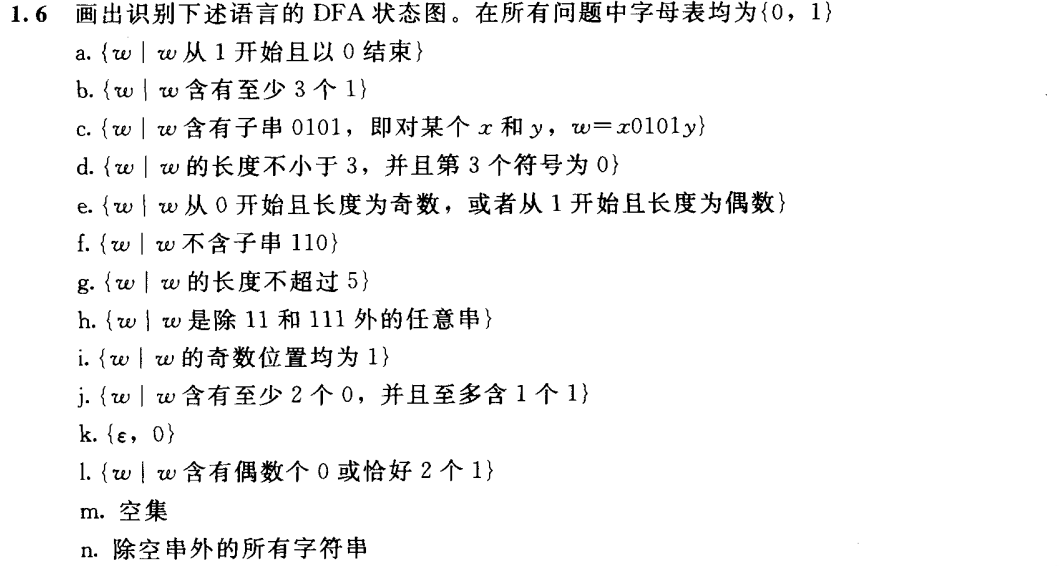
\includegraphics[width=\textwidth]{chapters/imgs/hw_1_6.png}
  \caption{}
  \label{fig:hw_1_6}
\end{figure}

\noindent\textbf{约定:}字母表 $\Sigma = \{0, 1\}$。所有 DFA 都是完备的,死状态用红色底色标出,接受态用双圆。

% ============================================================
% a. 从 1 开始且以 0 结束
% ============================================================
\subsubsection*{(a) $\{w \mid w$ 从 1 开始且以 0 结束$\}$}

状态:$q_0$ 起始(未读字符);$q_d$ 首字符为 0 的死状态;$q_1$ 首字符 1,当前末字符 1(非接受);$q_2$ 首字符 1,当前末字符 0(接受)。

\begin{center}
\begin{tikzpicture}[shorten >=1pt, auto, node distance=3cm, on grid]
    \node[state, initial]   (q0)              {$q_0$};
    \node[state]            (q1) [right=of q0] {$q_1$};
    \node[state, accepting] (q2) [right=of q1] {$q_2$};
    \node[state, dead]      (qd) [below=of q1] {$q_d$};
    \path[->]
        (q0) edge              node        {1}   (q1)
        (q0) edge              node [swap] {0}   (qd)
        (q1) edge [bend left]  node        {0}   (q2)
        (q2) edge [bend left]  node        {1}   (q1)
        (q1) edge [loop above] node        {1}   ()
        (q2) edge [loop above] node        {0}   ()
        (qd) edge [loop below] node        {0,1} ();
\end{tikzpicture}
\end{center}

% ============================================================
% b. 含至少 3 个 1
% ============================================================
\subsubsection*{(b) $\{w \mid w$ 含有至少 3 个 $1\}$}

按 1 的计数划分,3 饱和。

\begin{center}
\begin{tikzpicture}[shorten >=1pt, auto, node distance=2.6cm, on grid]
    \node[state, initial]    (q0)               {$q_0$};
    \node[state]             (q1) [right=of q0] {$q_1$};
    \node[state]             (q2) [right=of q1] {$q_2$};
    \node[state, accepting]  (q3) [right=of q2] {$q_3$};
    \path[->]
        (q0) edge              node {1}   (q1)
        (q1) edge              node {1}   (q2)
        (q2) edge              node {1}   (q3)
        (q0) edge [loop above] node {0}   ()
        (q1) edge [loop above] node {0}   ()
        (q2) edge [loop above] node {0}   ()
        (q3) edge [loop above] node {0,1} ();
\end{tikzpicture}
\end{center}

% ============================================================
% c. 含子串 0101
% ============================================================
\subsubsection*{(c) $\{w \mid w$ 含子串 $0101\}$}

跟踪匹配进度,失配时回到最长的已匹配前缀。关键回退:$q_1$(已匹配 0)读 0 保持 $q_1$;$q_3$(已匹配 010)读 0 退回 $q_1$(新 0 可能是新匹配开头)。

\begin{center}
\begin{tikzpicture}[shorten >=1pt, auto, node distance=2.5cm, on grid]
    \node[state, initial]    (q0)                    {$q_0$};
    \node[state]             (q1) [right=of q0]      {$q_1$};
    \node[state]             (q2) [right=of q1]      {$q_2$};
    \node[state]             (q3) [right=of q2]      {$q_3$};
    \node[state, accepting]  (q4) [right=of q3]      {$q_4$};
    \path[->]
        (q0) edge                  node {0}   (q1)
        (q1) edge                  node {1}   (q2)
        (q2) edge                  node {0}   (q3)
        (q3) edge                  node {1}   (q4)
        (q0) edge [loop above]     node {1}   ()
        (q1) edge [loop above]     node {0}   ()
        (q2) edge [bend left=40]   node {1}   (q0)
        (q3) edge [bend left=30]   node {0}   (q1)
        (q4) edge [loop above]     node {0,1} ();
\end{tikzpicture}
\end{center}

% ============================================================
% d. 长度 >= 3 且第 3 个符号为 0
% ============================================================
\subsubsection*{(d) $\{w \mid |w| \geq 3$ 且第 3 个符号为 $0\}$}

前三步按位置推进,第 3 个字符决定去向。

\begin{center}
\begin{tikzpicture}[shorten >=1pt, auto, node distance=2.6cm, on grid]
    \node[state, initial]    (q0)                 {$q_0$};
    \node[state]             (q1) [right=of q0]   {$q_1$};
    \node[state]             (q2) [right=of q1]   {$q_2$};
    \node[state, accepting]  (q3) [right=of q2]   {$q_3$};
    \node[state, dead]       (qd) [below=of q2]   {$q_d$};
    \path[->]
        (q0) edge              node        {0,1} (q1)
        (q1) edge              node        {0,1} (q2)
        (q2) edge              node        {0}   (q3)
        (q2) edge              node [swap] {1}   (qd)
        (q3) edge [loop above] node        {0,1} ()
        (qd) edge [loop below] node        {0,1} ();
\end{tikzpicture}
\end{center}

% ============================================================
% e. 从 0 开始且长度奇数,或从 1 开始且长度偶数
% ============================================================
\subsubsection*{(e) $\{w \mid w$ 从 0 开始且长度奇数,或从 1 开始且长度偶数$\}$}

空串不满足任一条件(空串无首字符)。5 个状态:$q_0$ 起始;$0E, 0O$(首 0,当前长度偶/奇);$1E, 1O$(首 1,当前长度偶/奇)。
接受:$0O$(首 0 + 奇长)、$1E$(首 1 + 偶长,但长度至少为 2)。

\begin{center}
\begin{tikzpicture}[shorten >=1pt, auto, node distance=2.8cm, on grid]
    \node[state, initial]              (q0)                   {$q_0$};
    \node[state]                       (zE) [above right=of q0] {$0E$};
    \node[state, accepting]            (zO) [right=of zE]       {$0O$};
    \node[state, accepting]            (oE) [below right=of q0] {$1E$};
    \node[state]                       (oO) [right=of oE]       {$1O$};
    \path[->]
        (q0) edge                 node        {0}   (zO)
        (q0) edge                 node [swap] {1}   (oO)
        (zO) edge [bend left=15]  node        {0,1} (zE)
        (zE) edge [bend left=15]  node        {0,1} (zO)
        (oO) edge [bend left=15]  node        {0,1} (oE)
        (oE) edge [bend left=15]  node        {0,1} (oO);
\end{tikzpicture}
\end{center}

\noindent 注:从 $q_0$ 读 0 后长度已为 1(奇),直接进入接受态 $0O$;读 1 后长度为 1(奇,不接受),进入 $1O$,再读一字符才到 $1E$ 接受。

% ============================================================
% f. 不含子串 110
% ============================================================
\subsubsection*{(f) $\{w \mid w$ 不含子串 $110\}$}

先画含 110 的 DFA,再翻转接受态。$q_0$(未匹配)、$q_1$(匹配 1)、$q_2$(匹配 11)、$q_3$(已含 110)。

\begin{center}
\begin{tikzpicture}[shorten >=1pt, auto, node distance=2.8cm, on grid]
    \node[state, initial, accepting]  (q0)                  {$q_0$};
    \node[state, accepting]           (q1) [right=of q0]    {$q_1$};
    \node[state, accepting]           (q2) [right=of q1]    {$q_2$};
    \node[state, dead]                (q3) [right=of q2]    {$q_3$};
    \path[->]
        (q0) edge                  node {1}   (q1)
        (q1) edge                  node {1}   (q2)
        (q2) edge                  node {0}   (q3)
        (q0) edge [loop above]     node {0}   ()
        (q1) edge [bend left=30]   node {0}   (q0)
        (q2) edge [loop above]     node {1}   ()
        (q3) edge [loop above]     node {0,1} ();
\end{tikzpicture}
\end{center}

% ============================================================
% g. 长度不超过 5
% ============================================================
\subsubsection*{(g) $\{w \mid |w| \leq 5\}$}

6 个接受态对应长度 $0, 1, \ldots, 5$,第 7 个状态为死态(长度 $\geq 6$)。

\begin{center}
\begin{tikzpicture}[shorten >=1pt, auto, node distance=1.9cm, on grid]
    \node[state, initial, accepting]  (q0)               {$q_0$};
    \node[state, accepting]           (q1) [right=of q0] {$q_1$};
    \node[state, accepting]           (q2) [right=of q1] {$q_2$};
    \node[state, accepting]           (q3) [right=of q2] {$q_3$};
    \node[state, accepting]           (q4) [right=of q3] {$q_4$};
    \node[state, accepting]           (q5) [right=of q4] {$q_5$};
    \node[state, dead]                (qd) [right=of q5] {$q_d$};
    \path[->]
        (q0) edge              node {0,1} (q1)
        (q1) edge              node {0,1} (q2)
        (q2) edge              node {0,1} (q3)
        (q3) edge              node {0,1} (q4)
        (q4) edge              node {0,1} (q5)
        (q5) edge              node {0,1} (qd)
        (qd) edge [loop above] node {0,1} ();
\end{tikzpicture}
\end{center}

% ============================================================
% h. 除 11 和 111 外的任意串
% ============================================================
\subsubsection*{(h) $\{w \mid w \neq 11$ 且 $w \neq 111\}$}

即 $\Sigma^* \setminus \{11, 111\}$。先识别 $\{11, 111\}$ 再取补。只需追踪"连续 1 的前缀长度 0/1/2/3"以及"是否已经出现过 0"。

\begin{center}
\begin{tikzpicture}[shorten >=1pt, auto, node distance=2.6cm, on grid]
    \node[state, initial, accepting]  (q0)                   {$q_0$};
    \node[state, accepting]           (q1) [right=of q0]     {$q_1$};
    \node[state]                      (q2) [right=of q1]     {$q_2$};
    \node[state]                      (q3) [right=of q2]     {$q_3$};
    \node[state, accepting]           (q4) [right=of q3]     {$q_4$};
    \node[state, accepting]           (qZ) [below=of q2]     {$q_Z$};
    \path[->]
        (q0) edge                 node        {1}   (q1)
        (q1) edge                 node        {1}   (q2)
        (q2) edge                 node        {1}   (q3)
        (q3) edge                 node        {0,1} (q4)
        (q0) edge [bend right=40] node [swap] {0}   (qZ)
        (q1) edge                 node [swap] {0}   (qZ)
        (q2) edge                 node        {0}   (qZ)
        (q3) edge [bend right=20] node        {0}   (qZ)
        (q4) edge [loop above]    node        {0,1} ()
        (qZ) edge [loop below]    node        {0,1} ();
\end{tikzpicture}
\end{center}

\noindent 状态含义:$q_0 = \varepsilon$(接受);$q_1 = 1$(接受,不等于 11 或 111);$q_2 = 11$(不接受);$q_3 = 111$(不接受);$q_4$ = 长度 $\geq 4$ 的纯 1 串或 $111$ 之后还有字符(接受);$q_Z$ = 任何阶段出现过 0,说明不是纯 1 串,肯定不等于 11 或 111(接受)。

% ============================================================
% i. 奇数位置均为 1
% ============================================================
\subsubsection*{(i) $\{w \mid w$ 的奇数位置均为 $1\}$}

位置从 1 开始数。奇数位必须是 1,偶数位随意。空串空位置集满足,接受。

\begin{center}
\begin{tikzpicture}[shorten >=1pt, auto, node distance=3cm, on grid]
    \node[state, initial, accepting]  (q0)               {$q_{\text{odd}}$};
    \node[state, accepting]           (q1) [right=of q0] {$q_{\text{even}}$};
    \node[state, dead]                (qd) [right=of q1] {$q_d$};
    \path[->]
        (q0) edge [bend left]     node        {1}   (q1)
        (q1) edge [bend left]     node        {0,1} (q0)
        (q0) edge                 node        {0}   (qd)
        (qd) edge [loop above]    node        {0,1} ();
\end{tikzpicture}
\end{center}

\noindent $q_{\text{odd}}$:下一读入位置是奇数,必须为 1;$q_{\text{even}}$:下一位置是偶数,0/1 都可;一旦奇数位读到 0 就进入死态。

% ============================================================
% j. 含至少 2 个 0 且至多 1 个 1
% ============================================================
\subsubsection*{(j) $\{w \mid w$ 含至少 2 个 0 且至多 1 个 $1\}$}

笛卡尔积:0 计数 $\{0, 1, \geq 2\}$ $\times$ 1 计数 $\{0, 1, \geq 2 \text{(死)}\}$。去掉 1 计数 $\geq 2$ 那列后只剩 2 列,加一个共用死态共 $3 \times 2 + 1 = 7$ 个状态(下面把同为死态的合并)。

\noindent 状态记作 $(i, j)$,$i$ = 0 的计数(0/1/2+),$j$ = 1 的计数(0/1)。接受 $(2, 0)$ 和 $(2, 1)$。

\begin{center}
\begin{tikzpicture}[shorten >=1pt, auto, node distance=2.8cm, on grid]
    \node[state, initial]    (a00)                      {$0,0$};
    \node[state]             (a10) [right=of a00]       {$1,0$};
    \node[state, accepting]  (a20) [right=of a10]       {$2,0$};
    \node[state]             (a01) [below=of a00]       {$0,1$};
    \node[state]             (a11) [below=of a10]       {$1,1$};
    \node[state, accepting]  (a21) [below=of a20]       {$2,1$};
    \node[state, dead]       (qd)  [below=of a11]       {$q_d$};
    \path[->]
        (a00) edge              node        {0}   (a10)
        (a10) edge              node        {0}   (a20)
        (a20) edge [loop above] node        {0}   ()
        (a01) edge              node        {0}   (a11)
        (a11) edge              node        {0}   (a21)
        (a21) edge [loop below] node        {0}   ()
        (a00) edge              node        {1}   (a01)
        (a10) edge              node        {1}   (a11)
        (a20) edge              node        {1}   (a21)
        (a01) edge              node [swap] {1}   (qd)
        (a11) edge              node [swap] {1}   (qd)
        (a21) edge              node        {1}   (qd)
        (qd)  edge [loop right] node        {0,1} ();
\end{tikzpicture}
\end{center}

% ============================================================
% k. {ε, 0}
% ============================================================
\subsubsection*{(k) $\{\varepsilon, 0\}$}

只接受空串和单字符 0。

\begin{center}
\begin{tikzpicture}[shorten >=1pt, auto, node distance=3cm, on grid]
    \node[state, initial, accepting]  (q0)               {$q_0$};
    \node[state, accepting]           (q1) [right=of q0] {$q_1$};
    \node[state, dead]                (qd) [right=of q1] {$q_d$};
    \path[->]
        (q0) edge              node        {0}   (q1)
        (q0) edge [bend right] node [swap] {1}   (qd)
        (q1) edge              node        {0,1} (qd)
        (qd) edge [loop above] node        {0,1} ();
\end{tikzpicture}
\end{center}

% ============================================================
% l. 含偶数个 0 或恰好 2 个 1
% ============================================================
\subsubsection*{(l) $\{w \mid w$ 含偶数个 0 或恰好 2 个 $1\}$}

并运算用笛卡尔积:$\{w \mid \#_0 \text{ 偶}\}$ 的 2 状态 DFA $\times$ $\{w \mid \#_1 = 2\}$ 的 4 状态 DFA = 8 状态。接受态:**至少一个分量是接受态**(并运算)。状态记为 $(p, k)$,$p \in \{E, O\}$(0 的奇偶),$k \in \{0, 1, 2, 3\}$(1 的计数,3 代表 $\geq 3$)。

\begin{center}
\begin{tikzpicture}[shorten >=1pt, auto, node distance=2.4cm, on grid]
    \node[state, initial, accepting]  (E0)                {$E,0$};
    \node[state, accepting]           (E1) [right=of E0]  {$E,1$};
    \node[state, accepting]           (E2) [right=of E1]  {$E,2$};
    \node[state, accepting]           (E3) [right=of E2]  {$E,3$};
    \node[state]                      (O0) [below=of E0]  {$O,0$};
    \node[state]                      (O1) [below=of E1]  {$O,1$};
    \node[state, accepting]           (O2) [below=of E2]  {$O,2$};
    \node[state]                      (O3) [below=of E3]  {$O,3$};
    \path[->]
        % 0 翻转 E/O
        (E0) edge [bend left=12]  node        {0} (O0)
        (O0) edge [bend left=12]  node        {0} (E0)
        (E1) edge [bend left=12]  node        {0} (O1)
        (O1) edge [bend left=12]  node        {0} (E1)
        (E2) edge [bend left=12]  node        {0} (O2)
        (O2) edge [bend left=12]  node        {0} (E2)
        (E3) edge [bend left=12]  node        {0} (O3)
        (O3) edge [bend left=12]  node        {0} (E3)
        % 1 计数 +1
        (E0) edge                 node        {1} (E1)
        (E1) edge                 node        {1} (E2)
        (E2) edge                 node        {1} (E3)
        (E3) edge [loop above]    node        {1} ()
        (O0) edge                 node [swap] {1} (O1)
        (O1) edge                 node [swap] {1} (O2)
        (O2) edge                 node [swap] {1} (O3)
        (O3) edge [loop below]    node        {1} ();
\end{tikzpicture}
\end{center}

\noindent 接受规则(并):$E$ 行全部接受(因为 0 偶);$O$ 行中只有 $(O, 2)$ 接受(1 恰好 2 个)。

% ============================================================
% m. 空集
% ============================================================
\subsubsection*{(m) 空集 $\varnothing$}

不接受任何串。只需一个非接受态带所有字符自环。

\begin{center}
\begin{tikzpicture}[shorten >=1pt, auto, node distance=3cm, on grid]
    \node[state, initial, dead]  (q0) {$q_0$};
    \path[->] (q0) edge [loop above] node {0,1} ();
\end{tikzpicture}
\end{center}

% ============================================================
% n. 除空串外的所有串
% ============================================================
\subsubsection*{(n) 除空串外的所有串 $\Sigma^+$}

起始态不接受(用于排除空串),读任一字符就进入永久接受态。

\begin{center}
\begin{tikzpicture}[shorten >=1pt, auto, node distance=3cm, on grid]
    \node[state, initial]    (q0)               {$q_0$};
    \node[state, accepting]  (q1) [right=of q0] {$q_1$};
    \path[->]
        (q0) edge              node {0,1} (q1)
        (q1) edge [loop above] node {0,1} ();
\end{tikzpicture}
\end{center}


\subsection*{1.7}

\begin{figure}[H]
  \centering
  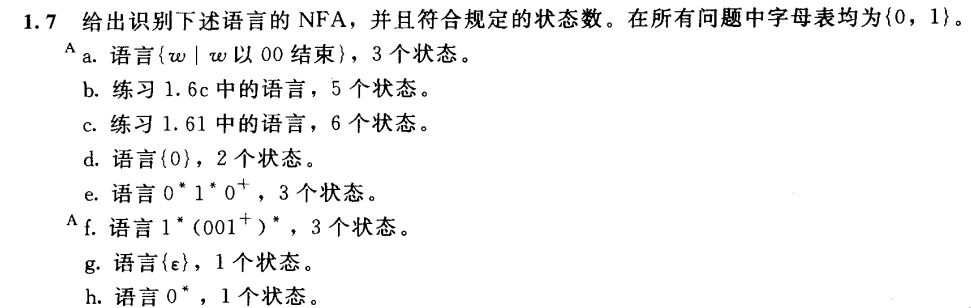
\includegraphics[width=\textwidth]{chapters/imgs/hw_1_7.png}
  \caption{}
  \label{fig:hw_1_7}
\end{figure}

\noindent\textbf{方法总结:}NFA 允许不完备的转移函数、对同一符号有多个去向、以及 $\varepsilon$ 转移。构造时常用技巧:(1) 用起始态自环"等待"匹配时机,由非确定性"猜"何时进入识别阶段;(2) 用 $\varepsilon$ 转移实现并运算和 Kleene 星号;(3) 缺失的转移即"拒绝当前分支"。

% ============================================================
% a. 以 00 结束 (3 状态)
% ============================================================
\subsubsection*{(a) $\{w \mid w$ 以 $00$ 结束$\}$,3 个状态}

$q_0$ 靠自环消耗任意前缀,非确定性地"猜"最后两个字符是 $00$ 并分支到 $q_1, q_2$。

\begin{center}
\begin{tikzpicture}[shorten >=1pt, auto, node distance=3cm, on grid]
    \node[state, initial]    (q0)                {$q_0$};
    \node[state]             (q1) [right=of q0]  {$q_1$};
    \node[state, accepting]  (q2) [right=of q1]  {$q_2$};
    \path[->]
        (q0) edge [loop above] node {0,1} ()
        (q0) edge              node {0}   (q1)
        (q1) edge              node {0}   (q2);
\end{tikzpicture}
\end{center}

% ============================================================
% b. 含子串 0101 (5 状态)
% ============================================================
\subsubsection*{(b) $\{w \mid w$ 含子串 $0101\}$,5 个状态}

与 1.6c 的 DFA 相比,NFA 无需设计失配回退 —— $q_0$ 自环"等"匹配时机。

\begin{center}
\begin{tikzpicture}[shorten >=1pt, auto, node distance=2.3cm, on grid]
    \node[state, initial]    (q0)                {$q_0$};
    \node[state]             (q1) [right=of q0]  {$q_1$};
    \node[state]             (q2) [right=of q1]  {$q_2$};
    \node[state]             (q3) [right=of q2]  {$q_3$};
    \node[state, accepting]  (q4) [right=of q3]  {$q_4$};
    \path[->]
        (q0) edge [loop above] node {0,1} ()
        (q0) edge              node {0}   (q1)
        (q1) edge              node {1}   (q2)
        (q2) edge              node {0}   (q3)
        (q3) edge              node {1}   (q4)
        (q4) edge [loop above] node {0,1} ();
\end{tikzpicture}
\end{center}

% ============================================================
% c. 含偶数个 0 或恰好 2 个 1 (6 状态)
% ============================================================
\subsubsection*{(c) 练习 1.6l 中的语言:偶数个 0 \emph{或} 恰好 2 个 1,6 个状态}

并运算用两条 $\varepsilon$ 转移从起始态分叉到两个独立小 NFA。

\begin{center}
\begin{tikzpicture}[shorten >=1pt, auto, node distance=2.6cm, on grid]
    \node[state, initial]              (s)                       {$s$};
    % 上分支: 偶数个 0 (2 状态)
    \node[state, accepting]            (E)  [above right=of s]   {$E$};
    \node[state]                       (O)  [right=of E]         {$O$};
    % 下分支: 恰好 2 个 1 (3 状态)
    \node[state]                       (p0) [below right=of s]   {$p_0$};
    \node[state]                       (p1) [right=of p0]        {$p_1$};
    \node[state, accepting]            (p2) [right=of p1]        {$p_2$};
    \path[->]
        (s)  edge                    node        {$\varepsilon$} (E)
        (s)  edge                    node [swap] {$\varepsilon$} (p0)
        (E)  edge [bend left=15]     node        {0}             (O)
        (O)  edge [bend left=15]     node        {0}             (E)
        (E)  edge [loop above]       node        {1}             ()
        (O)  edge [loop above]       node        {1}             ()
        (p0) edge                    node        {1}             (p1)
        (p1) edge                    node        {1}             (p2)
        (p0) edge [loop below]       node        {0}             ()
        (p1) edge [loop below]       node        {0}             ()
        (p2) edge [loop below]       node        {0}             ();
\end{tikzpicture}
\end{center}

\noindent 上分支:$E$ = 已读偶数个 0(接受),$O$ = 奇数个 0。下分支:$p_k$ = 已读 $k$ 个 1,$p_2$ 接受;一旦再读 1 就无路可走(被拒绝)。

% ============================================================
% d. {0} (2 状态)
% ============================================================
\subsubsection*{(d) 语言 $\{0\}$,2 个状态}

只接受单字符 0。读 1 或超出 1 字符都无路可走。

\begin{center}
\begin{tikzpicture}[shorten >=1pt, auto, node distance=3cm, on grid]
    \node[state, initial]    (q0)                {$q_0$};
    \node[state, accepting]  (q1) [right=of q0]  {$q_1$};
    \path[->]
        (q0) edge node {0} (q1);
\end{tikzpicture}
\end{center}

% ============================================================
% e. 0*1*0+ (3 状态)
% ============================================================
\subsubsection*{(e) 语言 $0^*1^*0^+$,3 个状态}

三个阶段对应三个状态。注意 $0^+$ 要求至少一个 0,所以 $q_2$ 必须**读到 0 才能进入**(不能用 $\varepsilon$ 跳进)。

\begin{center}
\begin{tikzpicture}[shorten >=1pt, auto, node distance=3cm, on grid]
    \node[state, initial]    (q0)                {$q_0$};
    \node[state]             (q1) [right=of q0]  {$q_1$};
    \node[state, accepting]  (q2) [right=of q1]  {$q_2$};
    \path[->]
        (q0) edge [loop above]  node {0}             ()
        (q1) edge [loop above]  node {1}             ()
        (q2) edge [loop above]  node {0}             ()
        (q0) edge               node {$\varepsilon$} (q1)
        (q1) edge               node {0}             (q2);
\end{tikzpicture}
\end{center}

\noindent $q_0$ 消耗 $0^*$ 前缀;$\varepsilon$ 进入 $q_1$ 消耗 $1^*$ 中间;读一个 0 进入 $q_2$ 接受,$q_2$ 再自环消耗剩余 0。

% ============================================================
% f. 1*(001+)* (3 状态)
% ============================================================
\subsubsection*{(f) 语言 $1^*(001^+)^*$,3 个状态}

$q_0$ 即接受态(对应已完成一个合法串,包括空串)。$q_0$ 自环吃掉任意多个 1;读 `00` 经由 $q_1$ 到 $q_2$;$q_2$ 必须\textbf{读至少一个 1} 才能返回 $q_0$,从而保证每个 $001$ 块末尾的 $1^+$ 至少有一个 1。

\begin{center}
\begin{tikzpicture}[shorten >=1pt, auto, node distance=3cm, on grid]
    \node[state, initial, accepting]  (q0)                {$q_0$};
    \node[state]                      (q1) [right=of q0]  {$q_1$};
    \node[state]                      (q2) [right=of q1]  {$q_2$};
    \path[->]
        (q0) edge [loop above]     node        {1}   ()
        (q0) edge                  node        {0}   (q1)
        (q1) edge                  node        {0}   (q2)
        (q2) edge [loop above]     node        {1}   ()
        (q2) edge [bend left=40]   node        {1}   (q0);
\end{tikzpicture}
\end{center}

\noindent 关键:$q_2$ 只能通过"读 1"离开(到 $q_0$ 或自身),这保证了每个 `00` 之后至少跟一个 1。NFA 的非确定性体现在:$q_2$ 读到一个 1 时,既可选择自环留在 $q_2$(继续延长当前块的 $1^+$),也可选择转移回 $q_0$(结束当前块或整个串)。

% ============================================================
% g. {ε} (1 状态)
% ============================================================
\subsubsection*{(g) 语言 $\{\varepsilon\}$,1 个状态}

只接受空串:起始态即接受态,无任何转移。

\begin{center}
\begin{tikzpicture}[shorten >=1pt, auto, node distance=3cm, on grid]
    \node[state, initial, accepting]  (q0)  {$q_0$};
\end{tikzpicture}
\end{center}

% ============================================================
% h. 0* (1 状态)
% ============================================================
\subsubsection*{(h) 语言 $0^*$,1 个状态}

起始态即接受态,加一个 0 自环。读到 1 无路可走。

\begin{center}
\begin{tikzpicture}[shorten >=1pt, auto, node distance=3cm, on grid]
    \node[state, initial, accepting]  (q0)  {$q_0$};
    \path[->] (q0) edge [loop right] node {0} ();
\end{tikzpicture}
\end{center}

\subsection*{1.11}

\begin{figure}[H]
  \centering
  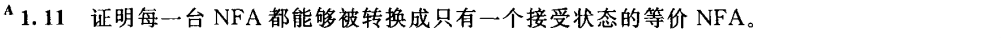
\includegraphics[width=\textwidth]{chapters/imgs/hw_1_11.png}
  \caption{}
  \label{fig:hw_1_11}
\end{figure}


\begin{figure}[H]
  \centering
  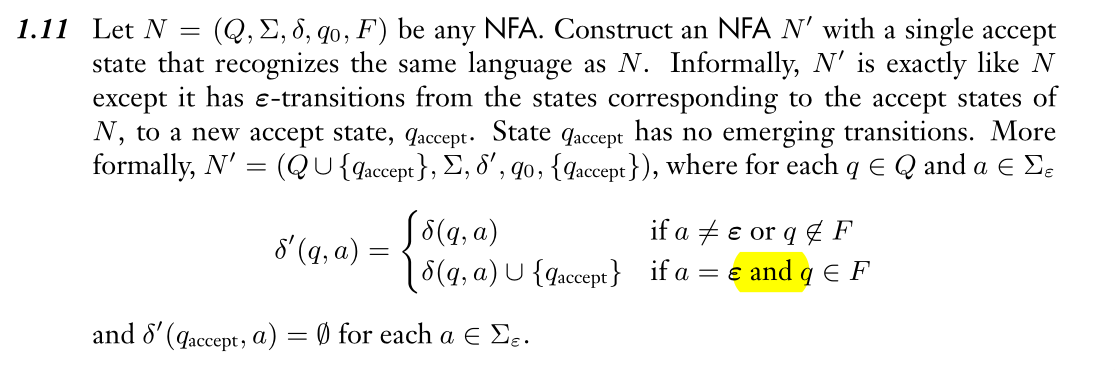
\includegraphics[width=\textwidth]{chapters/imgs/ans_p_1_11.png}
  \caption{}
  \label{fig:ans_p_1_11}
\end{figure}

\textbf{案：} 中文版此处翻译错误，$\delta'$的第二行中的两个条件应该为“且” 

\begin{figure}[H]
  \centering
  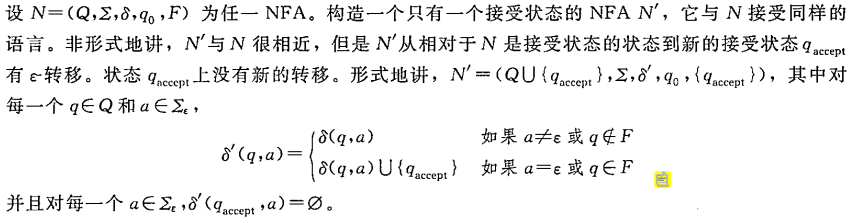
\includegraphics[width=\textwidth]{chapters/imgs/err_ans_p_1_11.png}
  \caption{}
  \label{fig:err_ans_p_1_11}
\end{figure}

\subsection*{1.13}

\begin{figure}[H]
  \centering
  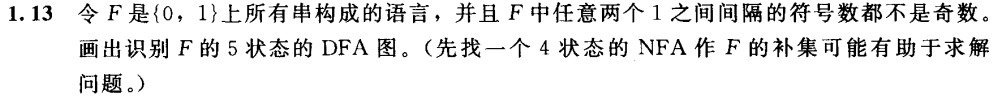
\includegraphics[width=\textwidth]{chapters/imgs/hw_1_13.png}
  \caption{}
  \label{fig:hw_1_13}
\end{figure}

\subsubsection*{1.13 $F = \{w \mid w$ 中任意两个 1 之间间隔的符号数都不是奇数$\}$}

\noindent\textbf{题意分析:}要求 $F$ 中的串,其中任意两个 1 之间的 0 的个数都是偶数(包括 0 个)。没有 1 或只有一个 1 的串自动满足(空真)。

\vspace{0.5em}
\noindent\textbf{策略:}按提示先构造识别 $\overline{F}$ 的 4 状态 NFA,再用子集构造转为 DFA,最后取补。

\paragraph{第一步:识别 $\overline{F}$ 的 4 状态 NFA。}
$\overline{F}$ = 存在某对 1,它们之间的 0 的个数是奇数。NFA 利用非确定性\textbf{猜}违反对的第一个 1,然后验证其后读了奇数个 0 再读到 1。

\begin{center}
\begin{tikzpicture}[shorten >=1pt, auto, node distance=2.8cm, on grid]
    \node[state, initial]    (q0)                 {$q_0$};
    \node[state]             (q1) [right=of q0]   {$q_1$};
    \node[state]             (q2) [right=of q1]   {$q_2$};
    \node[state, accepting]  (q3) [right=of q2]   {$q_3$};
    \path[->]
        (q0) edge [loop above]    node        {0,1} ()
        (q0) edge                 node        {1}   (q1)
        (q1) edge [bend left=15]  node        {0}   (q2)
        (q2) edge [bend left=15]  node        {0}   (q1)
        (q2) edge                 node        {1}   (q3)
        (q3) edge [loop above]    node        {0,1} ();
\end{tikzpicture}
\end{center}

\noindent 状态含义:$q_0$ = 读任意前缀;$q_1$ = 从猜到的第一个 1 起,已读\emph{偶数}个 0;$q_2$ = 已读\emph{奇数}个 0;$q_3$ = 奇数个 0 后读到第二个 1,违反对确认,接受。

\paragraph{第二步:子集构造转 DFA。}

\begin{center}
\begin{tabular}{c|c|c}
DFA 状态 & 读 0 & 读 1 \\
\hline
$A = \{q_0\}$                    & $\{q_0\} = A$               & $\{q_0, q_1\} = B$ \\
$B = \{q_0, q_1\}$              & $\{q_0, q_2\} = C$          & $\{q_0, q_1\} = B$ \\
$C = \{q_0, q_2\}$              & $\{q_0, q_1\} = B$          & $\{q_0, q_1, q_3\} = D$ \\
$D = \{q_0, q_1, q_3\}$         & $\{q_0, q_2, q_3\} = E$     & $\{q_0, q_1, q_3\} = D$ \\
$E = \{q_0, q_2, q_3\}$         & $\{q_0, q_1, q_3\} = D$     & $\{q_0, q_1, q_3\} = D$ \\
\end{tabular}
\end{center}

\noindent 得到 5 个可达状态。$\overline{F}$ 的接受态是含 $q_3$ 的状态:$D, E$。

\paragraph{第三步:取补得 $F$ 的 5 状态 DFA。}
将接受态翻转 —— $A, B, C$ 接受(未含违反对),$D, E$ 拒绝(已确认违反)。

\begin{center}
\begin{tikzpicture}[shorten >=1pt, auto, node distance=3cm, on grid]
    \node[state, initial, accepting]  (A)                       {$A$};
    \node[state, accepting]           (B)  [above right=of A]   {$B$};
    \node[state, accepting]           (C)  [below right=of A]   {$C$};
    \node[state, dead]                (D)  [right=of B]         {$D$};
    \node[state, dead]                (E)  [right=of C]         {$E$};
    \path[->]
        (A) edge [loop above]     node        {0}   ()
        (A) edge                  node        {1}   (B)
        (B) edge [bend left=15]   node        {0}   (C)
        (C) edge [bend left=15]   node        {0}   (B)
        (B) edge [loop above]     node        {1}   ()
        (C) edge                  node [swap] {1}   (E)
        (D) edge [bend left=15]   node        {0}   (E)
        (E) edge [bend left=15]   node        {0}   (D)
        (D) edge [loop above]     node        {1}   ()
        (E) edge                  node [swap] {1}   (D);
\end{tikzpicture}
\end{center}

\noindent\textbf{状态语义:}
\begin{itemize}
    \item $A$:尚未读到 1(空串 $\varepsilon$ 或全 0 串)
    \item $B$:上个 1 之后读了偶数个 0(含 0 个)—— 若串此刻结束,前面所有的 1-对间隔都合规
    \item $C$:上个 1 之后读了奇数个 0 —— 尚未确认违反(若后面不再有 1 也可接受)
    \item $D$:已经确认违反(在 $C$ 状态时读到过 1),当前距最后的 1 读了偶数个 0
    \item $E$:已经确认违反,当前距最后的 1 读了奇数个 0
\end{itemize}

\noindent 关键转移:$C \xrightarrow{1} E$ 是唯一"发生违反"的转移——在距上一个 1 奇数个 0 后又读到了一个 1。一旦进入 $\{D, E\}$ 就永远困在其中(死区)。

\subsection*{1.14}

\begin{figure}[H]
  \centering
  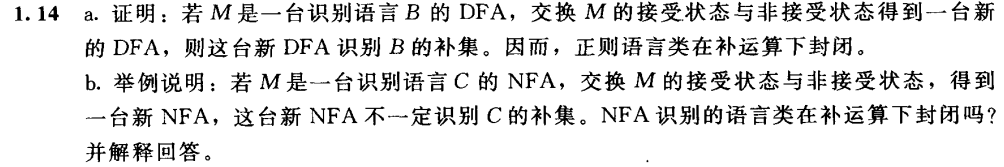
\includegraphics[width=\textwidth]{chapters/imgs/hw_1_14.png}
  \caption{}
  \label{fig:hw_1_14}
\end{figure}

\subsubsection*{解答}

先证明对 DFA 成立，再说明为什么对 NFA 直接交换接受状态与非接受状态并不正确。

\paragraph{DFA 情形.}
设
\[
    M = (Q, \Sigma, \delta, q_0, F)
\]
识别语言 $B$，即
\[
    B = L(M) = \{\, w \in \Sigma^* \mid \delta^*(q_0, w) \in F \,\}.
\]

构造新的 DFA
\[
    M' = (Q, \Sigma, \delta, q_0, Q \setminus F),
\]
也就是只交换接受状态与非接受状态，而保持转移函数不变。

对任意字符串 $w \in \Sigma^*$，由于 DFA 的计算路径唯一，
\[
    w \in L(M')
    \iff \delta^*(q_0, w) \in Q \setminus F
    \iff \delta^*(q_0, w) \notin F.
\]
另一方面，
\[
    \delta^*(q_0, w) \notin F
    \iff w \notin L(M)
    \iff w \notin B.
\]
因此
\[
    L(M') = \Sigma^* \setminus B = \overline{B}.
\]

所以，只要把一个识别 $B$ 的 DFA 的接受状态与非接受状态互换，就得到一个识别 $\overline{B}$ 的 DFA。于是，若 $B$ 是正则语言，则 $\overline{B}$ 也是正则语言。换言之，正则语言类在补运算下封闭。

\paragraph{NFA 情形.}
对于 NFA，直接交换接受状态与非接受状态不一定得到补语言。下面给出一个反例。

设字母表
\[
    \Sigma = \{a\}.
\]
构造 NFA
\[
    N = (Q, \Sigma, \delta, q_0, F),
\]
其中
\[
    Q = \{q_0, q_1\}, \qquad F = \{q_1\},
\]
转移为
\[
    \delta(q_0, a) = \{q_0, q_1\}, \qquad \delta(q_1, a) = \{q_1\}.
\]

这个 NFA 识别的语言是
\[
    C = \{a^n \mid n \geq 1\} = a^+.
\]
原因是：只要输入非空串，就可以在某一步从 $q_0$ 转到 $q_1$，并最终停在接受状态。

现在交换接受状态与非接受状态，得到
\[
    F' = Q \setminus F = \{q_0\}.
\]
设新 NFA 为
\[
    N' = (Q, \Sigma, \delta, q_0, F').
\]
由于对任意 $a^n$ 都可以始终停留在状态 $q_0$，所以
\[
    L(N') = a^*.
\]
但
\[
    \overline{C}
    = \Sigma^* \setminus a^+
    = \{\varepsilon\}.
\]
显然
\[
    L(N') = a^* \neq \{\varepsilon\} = \overline{C}.
\]

因此，对 NFA 直接交换接受状态与非接受状态，并不一定得到原语言的补集。

\paragraph{原因分析.}
DFA 的接受基于唯一计算路径，因此
\[
    w \in L(M)
    \iff \text{这唯一一条计算路径接受 } w.
\]
所以把接受态与非接受态交换后，恰好就把“接受”变成“拒绝”，把“拒绝”变成“接受”。

但 NFA 的接受条件是
\[
    w \in L(N)
    \iff \text{存在一条计算路径接受 } w.
\]
交换接受状态后，新 NFA 接受的是
\[
    \text{存在一条计算路径停在原来的非接受状态。}
\]
而补语言要求的是
\[
    w \in \overline{L(N)}
    \iff \text{不存在任何一条计算路径接受 } w,
\]
也就是
\[
    \forall \text{计算路径，都不接受}.
\]
这里“存在一条路径”与“所有路径都不接受”并不等价，所以不能通过简单交换终态来取补。

\paragraph{结论.}
虽然对 NFA 不能直接交换接受状态来取补，但 NFA 所识别的语言类仍然在补运算下封闭。因为任意 NFA 都可以先通过子集构造法转化为等价的 DFA，再对该 DFA 交换接受状态与非接受状态，即可得到补语言的识别器。$\blacksquare$



\subsection*{1.15}

\begin{figure}[H]
  \centering
  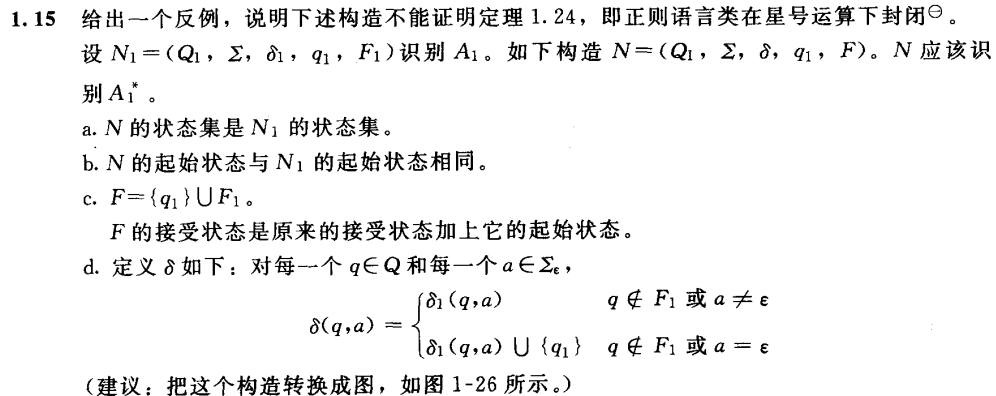
\includegraphics[width=\textwidth]{chapters/imgs/hw_1_15.png}
  \caption{}
  \label{fig:hw_1_15}
\end{figure}

这题中文版的第二版和第三版均存在翻译错误，下图\ref{fig:hw_1_15_en} 是英文版的题干

\begin{figure}[H]
  \centering
  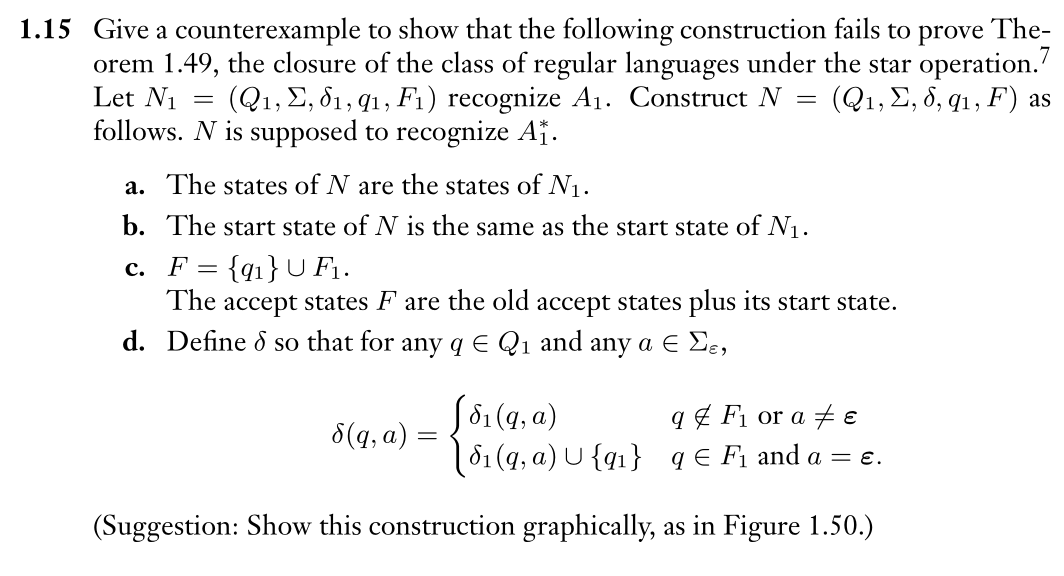
\includegraphics[width=\textwidth]{chapters/imgs/hw_1_15_en.png}
  \caption{}
  \label{fig:hw_1_15_en}
\end{figure}

\subsubsection*{解答}

这份证明的问题在于：所构造的新 NFA 并不一定识别 $A_1^*$。下面给出一个反例。

\paragraph{反例的选择.}
取
\[
    A_1 = a(ba)^*.
\]
令 $N_1$ 是识别 $A_1$ 的 NFA，其状态图如下：

\begin{center}
\begin{tikzpicture}[shorten >=1pt, auto, node distance=3.2cm, on grid]
    \node[state, initial]      (q1)                 {$q_1$};
    \node[state, accepting]    (q2) [right=of q1]   {$q_2$};
    \path[->]
        (q1) edge                  node        {a}   (q2)
        (q2) edge [bend left=18]   node        {b}   (q1);
\end{tikzpicture}
\end{center}

其中 $q_1$ 是开始状态，$q_2$ 是唯一接受状态。因此
\[
    L(N_1) = \{a(ba)^k \mid k \geq 0\} = a(ba)^* = A_1.
\]

\paragraph{按题中错误方法构造新 NFA.}
按照题目中的构造，新 NFA $N$ 的接受状态变为
\[
    F = \{q_1\} \cup F_1 = \{q_1, q_2\},
\]
并且因为 $q_2 \in F_1$，所以还要加入一条 $\varepsilon$-转移 $q_2 \to q_1$。于是得到下图：

\begin{center}
\begin{tikzpicture}[shorten >=1pt, auto, node distance=3.2cm, on grid]
    \node[state, initial, accepting]  (q1)                 {$q_1$};
    \node[state, accepting]           (q2) [right=of q1]   {$q_2$};
    \path[->]
        (q1) edge                     node        {a}              (q2)
        (q2) edge [bend left=18]      node        {b}              (q1)
        (q2) edge [bend right=18]     node[swap]  {$\varepsilon$}  (q1);
\end{tikzpicture}
\end{center}

\paragraph{说明该构造出错.}
在这个新 NFA 中，
\[
    q_1 \xrightarrow{a} q_2 \xrightarrow{b} q_1,
\]
而 $q_1$ 已经是接受状态，所以
\[
    ab \in L(N).
\]

但是
\[
    ab \notin A_1^*.
\]
这是因为 $A_1 = a(ba)^*$ 中的每个非空字符串都以 $a$ 开头并以 $a$ 结尾，因此 $A_1^*$ 中每个非空块也都以 $a$ 结尾，从而任意非空拼接结果仍以 $a$ 结尾。字符串 $ab$ 以 $b$ 结尾，所以不可能属于 $A_1^*$。

因此
\[
    L(N) \neq A_1^*.
\]
这就说明题目中的构造不能用来证明正则语言类对 Kleene 星号运算封闭。

\paragraph{错误的本质.}
问题出在它直接把原开始状态 $q_1$ 设成了接受状态。这样一来，只要某条路径在“尚未完整读完一个 $A_1$-块”时返回到了 $q_1$，机器就可能提前接受，从而识别出不属于 $A_1^*$ 的字符串。

正确的做法是：新建一个\textbf{新的开始接受状态}，并从它向旧开始状态加一条 $\varepsilon$-边；同时从每个旧接受状态向旧开始状态加 $\varepsilon$-边。这样才能正确识别 $A_1^*$。$\blacksquare$

\subsection*{1.17}

\begin{figure}[H]
  \centering
  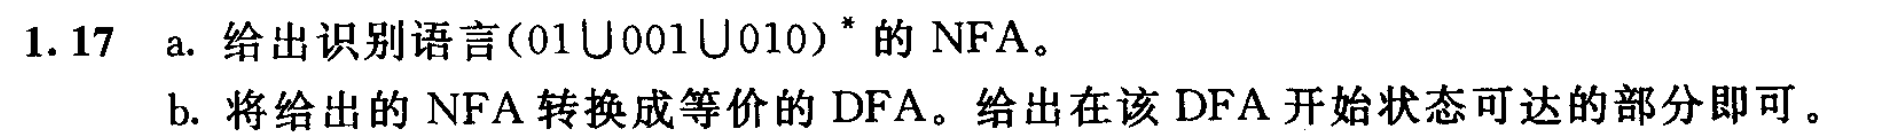
\includegraphics[width=\textwidth]{chapters/imgs/hw_1_17.png}
  \caption{}
  \label{fig:hw_1_17}
\end{figure}

\subsubsection*{解答}

\paragraph{识别 $(01 \cup 001 \cup 010)^*$ 的 NFA.}
按照正则表达式到 NFA 的标准构造，先分别构造识别 $01$、$001$、$010$ 的三个小 NFA，再用 $\varepsilon$ 边做并运算得到 $N_1$，最后在外层按星号构造得到 $N$。

\begin{center}
\begin{tikzpicture}[shorten >=1pt, auto, node distance=1.35cm and 1.7cm, on grid, scale=0.78, transform shape]
    \node[state, initial, accepting] (s)                              {$s$};
    \node[state]                     (u0) [right=2.1cm of s]          {$u_0$};

    \node[state]                     (a0) [above right=1.8cm and 1.6cm of u0] {$a_0$};
    \node[state]                     (a1) [right=of a0]               {$a_1$};
    \node[state, accepting]          (a2) [right=of a1]               {$a_2$};

    \node[state]                     (b0) [right=1.6cm of u0]         {$b_0$};
    \node[state]                     (b1) [right=of b0]               {$b_1$};
    \node[state]                     (b2) [right=of b1]               {$b_2$};
    \node[state, accepting]          (b3) [right=of b2]               {$b_3$};

    \node[state]                     (c0) [below right=1.8cm and 1.6cm of u0] {$c_0$};
    \node[state]                     (c1) [right=of c0]               {$c_1$};
    \node[state]                     (c2) [right=of c1]               {$c_2$};
    \node[state, accepting]          (c3) [right=of c2]               {$c_3$};
    \coordinate (toploop)    at ([yshift=1.10cm]a2.north);
    \coordinate (midloop)    at ([yshift=0.95cm]b3.north);
    \coordinate (bottomloop) at ([yshift=-1.05cm]c3.south);

    \node[draw, rounded corners=10pt, inner xsep=0.75cm, inner ysep=0.55cm,
          fit=(u0) (a0) (a2) (b0) (b3) (c0) (c3)] (None) {};
    \node[fill=white, inner sep=2pt] at (None.north west) {$N_1$};
    \node[draw, rounded corners=12pt, inner xsep=0.85cm, inner ysep=0.75cm,
          fit=(s) (None)] (N) {};
    \node[fill=white, inner sep=2pt] at (N.north west) {$N$};

    \path[->]
        (s)  edge                       node[fill=white, inner sep=1pt, above] {$\varepsilon$} (u0)

        (u0) edge                       node[fill=white, inner sep=1pt, above left] {$\varepsilon$} (a0)
        (u0) edge                       node[fill=white, inner sep=1pt, above]      {$\varepsilon$} (b0)
        (u0) edge                       node[fill=white, inner sep=1pt, below left] {$\varepsilon$} (c0)

        (a0) edge                       node[fill=white, inner sep=1pt, above] {0} (a1)
        (a1) edge                       node[fill=white, inner sep=1pt, above] {1} (a2)

        (b0) edge                       node[fill=white, inner sep=1pt, above] {0} (b1)
        (b1) edge                       node[fill=white, inner sep=1pt, above] {0} (b2)
        (b2) edge                       node[fill=white, inner sep=1pt, above] {1} (b3)

        (c0) edge                       node[fill=white, inner sep=1pt, above] {0} (c1)
        (c1) edge                       node[fill=white, inner sep=1pt, above] {1} (c2)
        (c2) edge                       node[fill=white, inner sep=1pt, above] {0} (c3);

    \draw[->]
        (a2.north) to[out=95, in=25] node[fill=white, inner sep=1pt, above] {$\varepsilon$} (toploop)
                   to[out=205, in=95] (u0.north);
    \draw[->]
        (b3.north) to[out=105, in=15] node[fill=white, inner sep=1pt, above] {$\varepsilon$} (midloop)
                   to[out=195, in=65] (u0.north east);
    \draw[->]
        (c3.south) to[out=-100, in=-25] node[fill=white, inner sep=1pt, below] {$\varepsilon$} (bottomloop)
                   to[out=155, in=-75] (u0.south);
\end{tikzpicture}
\end{center}

\noindent 其中 $N_1$ 识别 $01 \cup 001 \cup 010$，上、中、下三条分支分别识别 $01$、$001$、$010$。外层 $N$ 的新开始状态 $s$ 同时是接受状态，因此接受空串；从 $s$ 到 $u_0$ 的 $\varepsilon$ 边进入 $N_1$，从 $N_1$ 的接受状态回到 $u_0$ 的 $\varepsilon$ 边允许重复读下一个块。

\paragraph{子集构造得到的等价 DFA.}
为了得到较小的 DFA，可以先把上面的构造 NFA 化简为只记录“当前匹配到块内哪个前缀”的四状态 NFA。设该 NFA 的状态为 $q_0,q_1,q_2,q_3$，其中 $q_0$ 是开始状态和接受状态，并有如下含义：
\begin{center}
\begin{tabular}{c|l}
状态 & 含义 \\
\hline
$q_0$ & 当前正好停在块边界，可以接受；\\
$q_1$ & 已经读到某个块的前缀 $0$；\\
$q_2$ & 已经读到某个块的前缀 $00$；\\
$q_3$ & 已经读到某个块的前缀 $01$，还可继续读 $0$ 形成 $010$。
\end{tabular}
\end{center}

对这个 NFA 做子集构造时，DFA 的每个状态都是一个 NFA 状态集合。只保留从开始集合 $\{q_0\}$ 出发能够到达的集合，得到：
\begin{center}
\begin{tabular}{c|c|l}
DFA 状态 & NFA 状态集合 & 为什么会出现 \\
\hline
$A$ & $\{q_0\}$ & 开始集合\\
$B$ & $\{q_1\}$ & $A$ 读 $0$\\
$C$ & $\{q_2\}$ & $B$ 读 $0$\\
$D$ & $\{q_0,q_3\}$ & $B$ 或 $F$ 读 $1$\\
$E$ & $\{q_0,q_1\}$ & $D$ 读 $0$\\
$F$ & $\{q_1,q_2\}$ & $E$ 读 $0$\\
$G$ & $\emptyset$ & 无合法转移时进入的死状态
\end{tabular}
\end{center}

它们之间的转移由逐点取并得到：
\begin{center}
\begin{tabular}{c|cc}
状态 & $0$ & $1$ \\
\hline
$A$ & $B$ & $G$ \\
$B$ & $C$ & $D$ \\
$C$ & $G$ & $A$ \\
$D$ & $E$ & $G$ \\
$E$ & $F$ & $D$ \\
$F$ & $C$ & $D$ \\
$G$ & $G$ & $G$
\end{tabular}
\end{center}
因为原 NFA 的唯一接受态是 $q_0$，所以 DFA 中所有包含 $q_0$ 的状态都是接受状态，即 $A,D,E$；$G=\emptyset$ 是死状态。对应的 DFA 如下。

\begin{center}
\begin{tikzpicture}[shorten >=1pt, auto, on grid]
    \node[state, initial, accepting]  (A)                       {$A$};
    \node[state]                      (B)  [right=2.9cm of A]   {$B$};
    \node[state]                      (C)  [right=2.9cm of B]   {$C$};
    \node[state, dead]                (G)  [right=3.2cm of C]   {$G$};
    \node[state, accepting]           (E)  [below=2.8cm of A]   {$E$};
    \node[state, accepting]           (D)  [below=2.8cm of B]   {$D$};
    \node[state]                      (F)  [below=2.8cm of C]   {$F$};

    \path[->]
        (A) edge                      node[fill=white, inner sep=1pt, above] {0}   (B)
        (A) edge [bend left=18]       node[fill=white, inner sep=1pt, above] {1}   (G)

        (B) edge                      node[fill=white, inner sep=1pt, above] {0}   (C)
        (B) edge                      node[fill=white, inner sep=1pt, left]  {1}   (D)

        (C) edge [bend left=18]       node[fill=white, inner sep=1pt, above] {1}   (A)
        (C) edge                      node[fill=white, inner sep=1pt, above] {0}   (G)

        (D) edge [bend left=10]       node[fill=white, inner sep=1pt, above] {0}   (E)
        (D) edge [bend left=10]       node[fill=white, inner sep=1pt, below] {1}   (G)

        (E) edge [bend left=10]       node[fill=white, inner sep=1pt, above] {1}   (D)
        (E) edge [bend right=18]      node[fill=white, inner sep=1pt, below] {0}   (F)

        (F) edge                      node[fill=white, inner sep=1pt, right] {0}   (C)
        (F) edge [bend left=10]       node[fill=white, inner sep=1pt, below] {1}   (D)

        (G) edge [loop right]         node[fill=white, inner sep=1pt]        {0,1} ();
\end{tikzpicture}
\end{center}

\subsection*{1.19}

\begin{figure}[H]
  \centering
  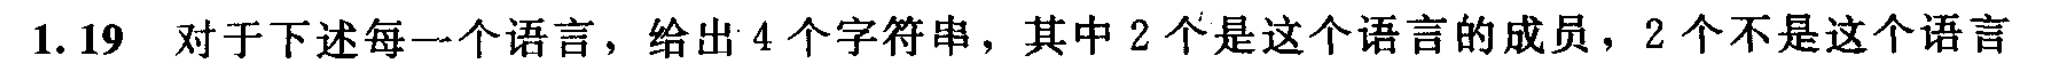
\includegraphics[width=\textwidth]{chapters/imgs/hw_1_19_p1.png}
  \caption{}
  \label{fig:hw_1_19_p1}
\end{figure}

\begin{figure}[H]
  \centering
  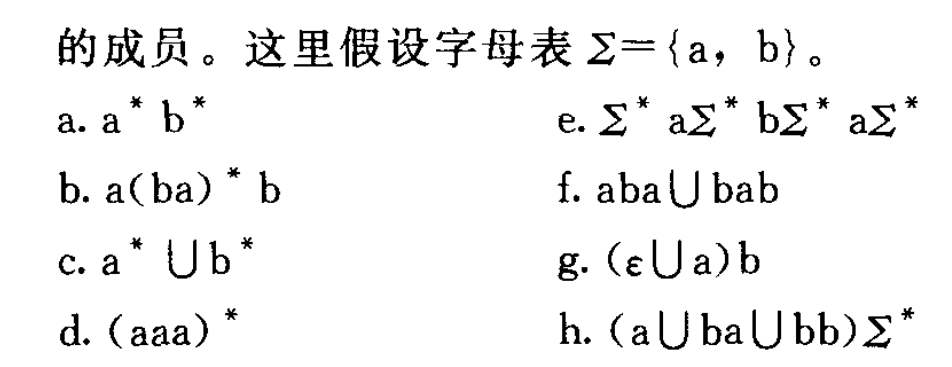
\includegraphics[width=\textwidth]{chapters/imgs/hw_1_19_p2.png}
  \caption{}
  \label{fig:hw_1_19_p2}
\end{figure}

\subsubsection*{解答}

下面给出每个语言的两个成员和两个非成员。这里约定字母表为 $\Sigma=\{a,b\}$。

\begin{center}
\renewcommand{\arraystretch}{1.3}
\begin{tabular}{c|c|c|c}
题号 & 语言 & 属于该语言的字符串 & 不属于该语言的字符串 \\
\hline
(a) & $a^*b^*$ & $\varepsilon,\ aaabbb$ & $ba,\ abab$ \\
(b) & $a(ba)^*b$ & $ab,\ abab$ & $\varepsilon,\ aab$ \\
(c) & $a^* \cup b^*$ & $aaa,\ bb$ & $ab,\ ba$ \\
(d) & $(aaa)^*$ & $\varepsilon,\ aaaaaa$ & $a,\ aa$ \\
(e) & $\Sigma^*a\Sigma^*b\Sigma^*a\Sigma^*$ & $aba,\ baaba$ & $\varepsilon,\ aab$ \\
(f) & $aba \cup bab$ & $aba,\ bab$ & $\varepsilon,\ ab$ \\
(g) & $(\varepsilon \cup a)b$ & $b,\ ab$ & $\varepsilon,\ a$ \\
(h) & $(a \cup ba \cup bb)\Sigma^*$ & $a,\ ba$ & $\varepsilon,\ b$ \\
\end{tabular}
\end{center}

\noindent 其中 (e) 要求字符串中存在一个按顺序出现的子序列 $a,b,a$；例如 $baaba$ 中第 $2,4,5$ 个字符可取为 $a,b,a$。而 (h) 表示字符串必须以 $a$、$ba$ 或 $bb$ 开头，所以空串和单独的 $b$ 都不属于该语言。

\subsection*{1.30}

\begin{figure}[H]
  \centering
  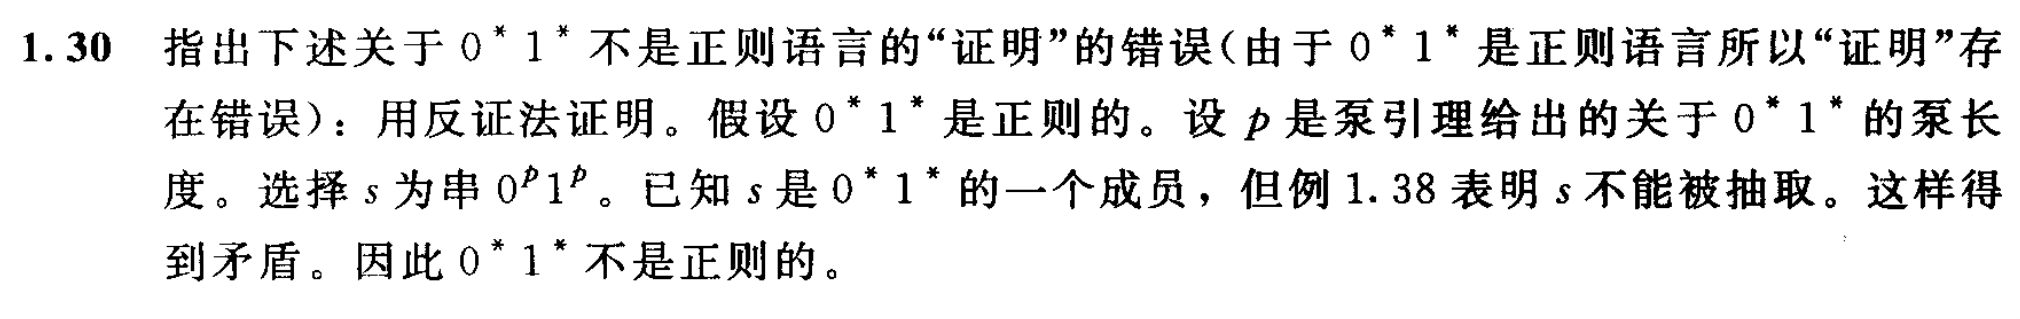
\includegraphics[width=\textwidth]{chapters/imgs/hw_1_30.png}
  \caption{}
  \label{fig:hw_1_30}
\end{figure}

\subsubsection*{解答}

该证明的错误在于混淆了两个不同的语言。语言
\[
    0^*1^*=\{0^m1^n \mid m,n\ge 0\}
\]
本身由正则表达式 $0^*1^*$ 描述，因而是正则语言，不可能由泵引理推出其非正则性。

错误发生在把例 1.38 中关于
\[
    B=\{0^n1^n \mid n\ge 0\}
\]
的结论用于 $0^*1^*$。对于 $B$，字符串 $0^p1^p$ 不能被泵，是因为泵动会破坏 $0$ 与 $1$ 的数量相等；但 $0^*1^*$ 并不要求二者数量相等，只要求所有 $0$ 在所有 $1$ 之前。

事实上，取
\[
    s=0^p1^p \in 0^*1^*,
\]
可作分解
\[
    x=\varepsilon,\qquad y=0,\qquad z=0^{p-1}1^p.
\]
于是对任意 $i\ge 0$，
\[
    xy^iz=0^{p-1+i}1^p \in 0^*1^*.
\]
因此该字符串在语言 $0^*1^*$ 中是可以被泵的。

泵引理用于证明非正则时，必须证明：存在某个选定的 $s\in A$，使得对所有满足条件的分解 $s=xyz$，都能找到 $i\ge 0$ 令 $xy^iz\notin A$。题中证明只借用了 $B=\{0^n1^n\mid n\ge 0\}$ 的结论，而该结论不能迁移到约束不同的语言 $0^*1^*$。$\blacksquare$

\subsubsection*{方法整理}

证明一个语言正则，通常采用构造法。也就是说，给出下列任意一种等价描述即可：
\[
    \text{正则表达式}\quad\Longleftrightarrow\quad
    \text{NFA}\quad\Longleftrightarrow\quad
    \text{DFA}.
\]
因此，若能直接写出正则表达式，或构造出识别该语言的 NFA/DFA，就已经证明了该语言正则。例如 $0^*1^*$ 由正则表达式本身描述，所以正则。

另一种常用方法是使用正则语言的闭包性质。已知正则语言类在并、连接、星号、补、交、差、逆、同态和逆同态等运算下封闭。因此，如果目标语言可由已知正则语言经过这些运算得到，也可推出其正则性。

证明一个语言非正则，则通常用反证法：先假设该语言正则，再推出矛盾。常用工具有：
\begin{enumerate}[label=(\arabic*), leftmargin=2.5em]
    \item 泵引理：设语言正则，取足够长且结构受限的字符串 $s$，证明对任意合法分解 $s=xyz$，总能选择某个 $i$ 使 $xy^iz$ 离开该语言。
    \item 闭包性质反证：若假设 $A$ 正则，则通过与某个正则语言求交、取差、同态等操作得到一个已知非正则语言，从而矛盾。
    \item 区分串方法：构造无限多个两两可区分的前缀，说明任何 DFA 都需要无限多个状态，因此语言非正则。
\end{enumerate}

需要注意，泵引理给出的是正则语言的必要条件，而不是充分条件。其逻辑形式是
\[
    A\text{ 正则}\quad\Longrightarrow\quad A\text{ 满足泵引理}.
\]
因此可以使用逆否命题
\[
    A\text{ 不满足泵引理}\quad\Longrightarrow\quad A\text{ 非正则},
\]
但不能反过来认为
\[
    A\text{ 满足泵引理}\quad\Longrightarrow\quad A\text{ 正则}.
\]
所以，泵引理是证明非正则的工具，而不是证明正则的工具。证明正则时应给出 RE、NFA、DFA，或把语言化归为正则语言闭包运算的结果。

\subsection*{1.32}

\begin{figure}[H]
  \centering
  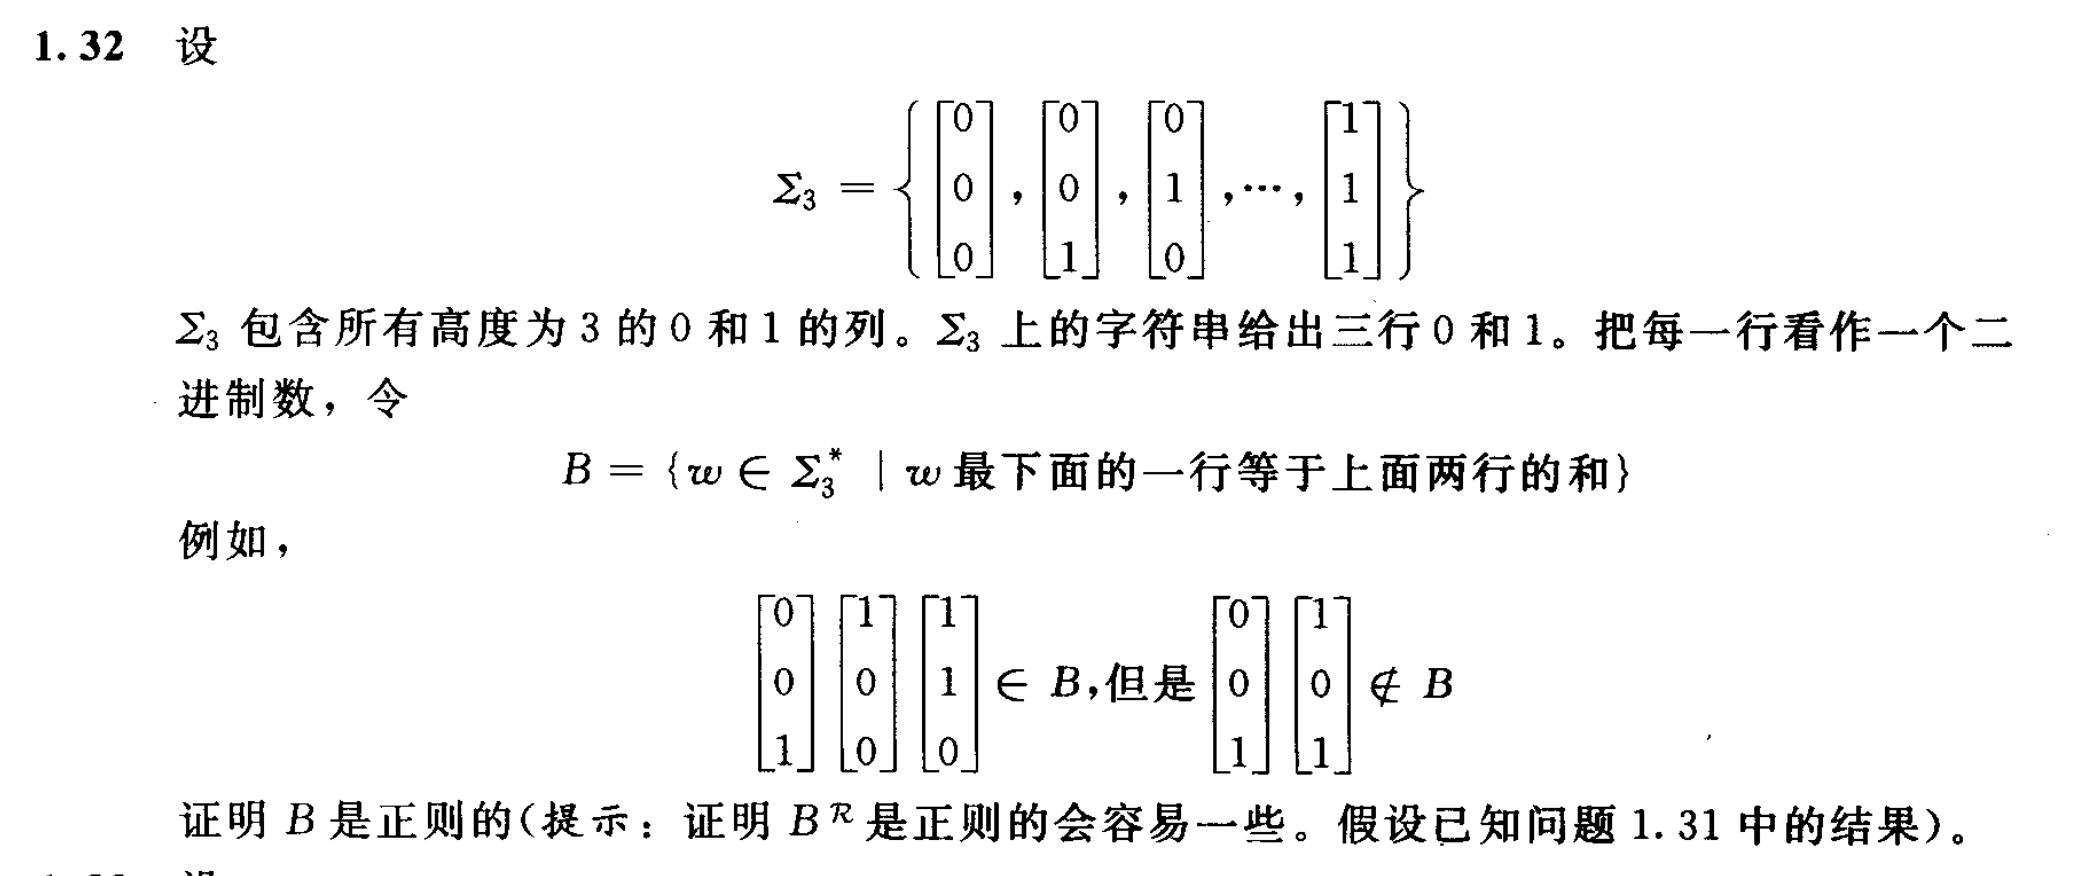
\includegraphics[width=\textwidth]{chapters/imgs/hw_1_32.png}
  \caption{}
  \label{fig:hw_1_32}
\end{figure}

\subsubsection*{证明}

二进制加法应从最低位向最高位检查。故先证明反转语言 $B^R$ 正则，再由正则语言对反转封闭推出 $B$ 正则。

设输入字母为三位列
\[
    \begin{bmatrix}
        a\\ b\\ c
    \end{bmatrix},
    \qquad a,b,c\in\{0,1\},
\]
分别表示两个加数与和的对应二进制位。在 $B^R$ 中，读入顺序正是从最低位到最高位，所以只需记录当前进位。

构造 DFA
\[
    M=(Q,\Sigma_3,\delta,q_0,F),
\]
其中
\[
    Q=\{q_0,q_1,q_d\},\qquad F=\{q_0\}.
\]
状态 $q_0,q_1$ 分别表示当前进位为 $0,1$，而 $q_d$ 为死状态。对 $r\in\{0,1\}$ 与任意列字母
\[
    \sigma=
    \begin{bmatrix}
        a\\ b\\ c
    \end{bmatrix},
\]
定义转移如下：若
\[
    c\equiv a+b+r \pmod 2,
\]
则
\[
    \delta(q_r,\sigma)
    =
    q_{\left\lfloor (a+b+r)/2\right\rfloor};
\]
否则令 $\delta(q_r,\sigma)=q_d$。并且对一切 $\sigma\in\Sigma_3$，
\[
    \delta(q_d,\sigma)=q_d.
\]

该 DFA 恰好逐位验证二进制加法，并把进位传递到下一列。输入结束时接受当且仅当最终进位为 $0$，即当前状态为 $q_0$。因此 $B^R$ 是正则语言。由于正则语言对反转封闭，
\[
    B=(B^R)^R
\]
也是正则语言。$\blacksquare$

\paragraph{解释.}
这个证明的核心是找出二进制加法检查中真正需要记住的信息。若从右向左读，即从最低位向最高位读，那么已经读过的低位对后续检查的影响只体现为当前进位。进位只有两种可能，$0$ 或 $1$，所以这是有限信息，可以由 DFA 的有限状态记录。

具体地，DFA 处在 $q_r$ 时表示“到目前为止读过的低位都合法，且传给下一位的进位为 $r$”。读入一列
\[
    \begin{bmatrix}
        a\\ b\\ c
    \end{bmatrix}
\]
后，DFA 检查 $c$ 是否等于 $a+b+r$ 的末位。如果不是，就进入死状态；如果是，就把状态更新为新的进位
\[
    \left\lfloor \frac{a+b+r}{2}\right\rfloor.
\]
因此 DFA 并不需要记住已经读过的全部数字，只需要记住一个有限状态：进位是否为 $1$。这正是该语言正则的原因。

\subsection*{1.34}

\begin{figure}[H]
  \centering
  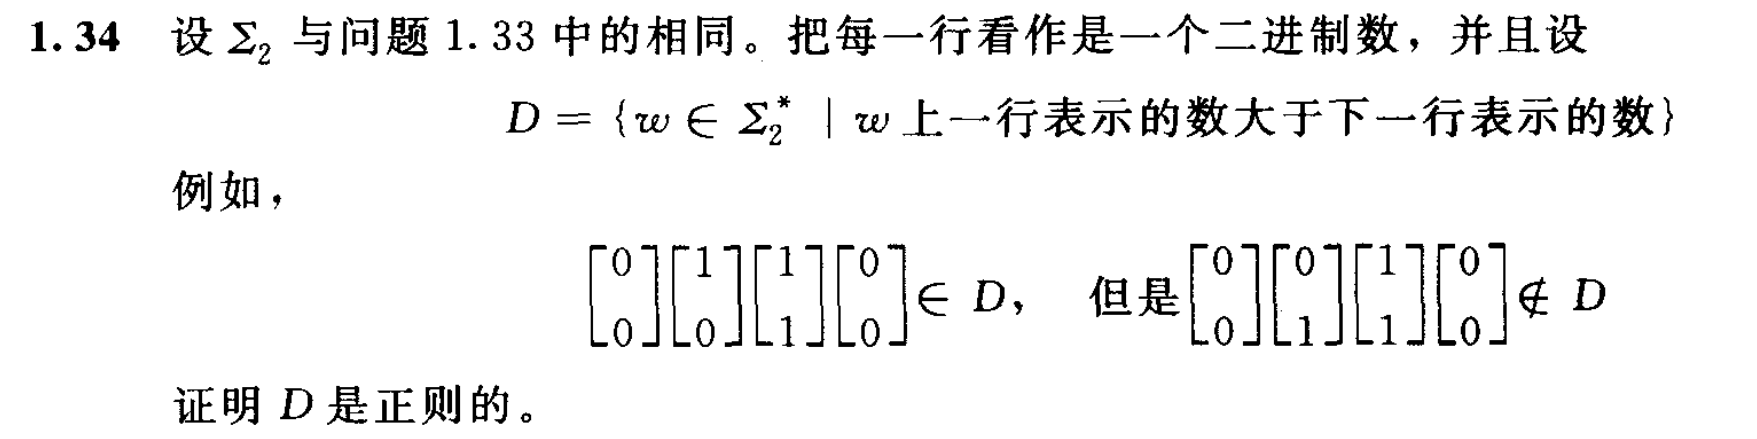
\includegraphics[width=\textwidth]{chapters/imgs/hw_1_34.png}
  \caption{}
  \label{fig:hw_1_34}
\end{figure}

\subsubsection*{证明}

设字母表为
\[
    \Sigma_2=
    \left\{
    \begin{bmatrix}0\\0\end{bmatrix},
    \begin{bmatrix}0\\1\end{bmatrix},
    \begin{bmatrix}1\\0\end{bmatrix},
    \begin{bmatrix}1\\1\end{bmatrix}
    \right\}.
\]
字符串
\[
    w=
    \begin{bmatrix}a_1\\ b_1\end{bmatrix}
    \begin{bmatrix}a_2\\ b_2\end{bmatrix}
    \cdots
    \begin{bmatrix}a_n\\ b_n\end{bmatrix}
\]
表示两行二进制数 $a_1a_2\cdots a_n$ 与 $b_1b_2\cdots b_n$。从左向右比较二者时，大小关系由最左边第一个不同位决定。

构造 DFA
\[
    M=(Q,\Sigma_2,\delta,q_=,F),
\]
其中
\[
    Q=\{q_=,q_>,q_<\},\qquad F=\{q_>\}.
\]
状态 $q_=$ 表示目前为止两行相等，$q_>$ 表示已经确定上面一行较大，$q_<$ 表示已经确定上面一行较小。

在状态 $q_=$ 时，定义
\[
\begin{aligned}
    \delta\left(q_=,\begin{bmatrix}0\\0\end{bmatrix}\right)&=q_=,
    &
    \delta\left(q_=,\begin{bmatrix}1\\1\end{bmatrix}\right)&=q_=,\\
    \delta\left(q_=,\begin{bmatrix}1\\0\end{bmatrix}\right)&=q_>,
    &
    \delta\left(q_=,\begin{bmatrix}0\\1\end{bmatrix}\right)&=q_<.
\end{aligned}
\]
一旦已经确定大小关系，后续位不再改变结果。因此对任意 $\sigma\in\Sigma_2$，
\[
    \delta(q_>,\sigma)=q_>,
    \qquad
    \delta(q_<,\sigma)=q_<.
\]

该 DFA 恰好记录从左至右比较时所需的有限信息：尚未分出大小、已经上大于下、已经上小于下。最终接受当且仅当最左边第一个不同位为
\[
    \begin{bmatrix}1\\0\end{bmatrix},
\]
即上面一行表示的二进制数大于下面一行。因此 $L(M)=D$，故 $D$ 是正则语言。$\blacksquare$

\subsection*{1.35}

\begin{figure}[H]
  \centering
  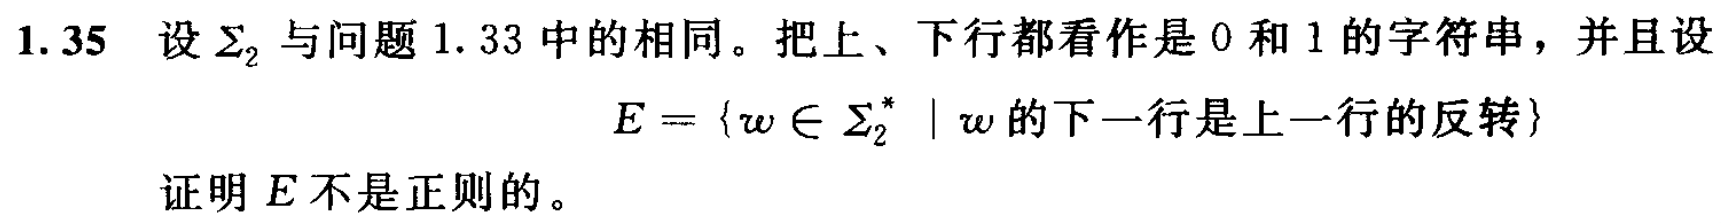
\includegraphics[width=\textwidth]{chapters/imgs/hw_1_35.png}
  \caption{}
  \label{fig:hw_1_35}
\end{figure}

\subsubsection*{证明}

设
\[
    \Sigma_2=
    \left\{
    \begin{bmatrix}0\\0\end{bmatrix},
    \begin{bmatrix}0\\1\end{bmatrix},
    \begin{bmatrix}1\\0\end{bmatrix},
    \begin{bmatrix}1\\1\end{bmatrix}
    \right\}.
\]
若
\[
    w=
    \begin{bmatrix}a_1\\ b_1\end{bmatrix}
    \begin{bmatrix}a_2\\ b_2\end{bmatrix}
    \cdots
    \begin{bmatrix}a_n\\ b_n\end{bmatrix},
\]
则 $w\in E$ 当且仅当
\[
    b_1b_2\cdots b_n=a_na_{n-1}\cdots a_1.
\]

用泵引理反证。假设 $E$ 正则，令 $p$ 为其泵长度。取
\[
    s=
    \begin{bmatrix}0\\1\end{bmatrix}^{p}
    \begin{bmatrix}1\\0\end{bmatrix}^{p}.
\]
其上行是 $0^p1^p$，下行是 $1^p0^p=(0^p1^p)^R$，故 $s\in E$，且 $|s|=2p\ge p$。

由泵引理，存在分解 $s=xyz$，满足
\[
    |xy|\le p,\qquad |y|>0,
\]
并且对所有 $i\ge 0$，有 $xy^iz\in E$。由于 $|xy|\le p$，子串 $y$ 完全位于前 $p$ 个字母中，所以
\[
    y=
    \begin{bmatrix}0\\1\end{bmatrix}^{k}
    \qquad(k>0).
\]
令 $i=0$，得到
\[
    xz=
    \begin{bmatrix}0\\1\end{bmatrix}^{p-k}
    \begin{bmatrix}1\\0\end{bmatrix}^{p}.
\]
此时上行是 $0^{p-k}1^p$，下行是 $1^{p-k}0^p$。然而
\[
    (0^{p-k}1^p)^R=1^p0^{p-k}
    \ne
    1^{p-k}0^p.
\]
故 $xz\notin E$，与泵引理要求 $xy^0z\in E$ 矛盾。因此 $E$ 不是正则语言。$\blacksquare$

\paragraph{解释.}
该语言要求下行等于上行的反转。也就是说，自动机读到前面的上行信息后，必须在后面以相反顺序逐位比较。随着输入长度增加，需要保存的前缀可以任意长；而 DFA 只有有限多个状态，不能保存任意长的前缀信息。这就是 $E$ 非正则的本质原因。

这里并不是只考察了某一种特殊分解。泵引理要求对任意满足 $|xy|\le p$、$|y|>0$ 的分解都能泵。我们选取的
\[
    s=
    \begin{bmatrix}0\\1\end{bmatrix}^{p}
    \begin{bmatrix}1\\0\end{bmatrix}^{p}
\]
有一个关键性质：它的前 $p$ 个符号全都是
\[
    \begin{bmatrix}0\\1\end{bmatrix}.
\]
因此无论合法分解 $s=xyz$ 怎样选，只要 $|xy|\le p$ 且 $|y|>0$，子串 $y$ 都必然具有形式
\[
    y=
    \begin{bmatrix}0\\1\end{bmatrix}^{k}
    \qquad(k>0).
\]
所以证明中令 $y=\begin{bmatrix}0\\1\end{bmatrix}^{k}$ 并不是任取一种情况，而是概括了所有合法分解。随后取 $i=0$，对任意这样的 $k>0$ 都会破坏上下两行的反转关系，故得到的矛盾满足泵引理反证所需的量词结构。

\subsection*{1.36}

\begin{figure}[H]
  \centering
  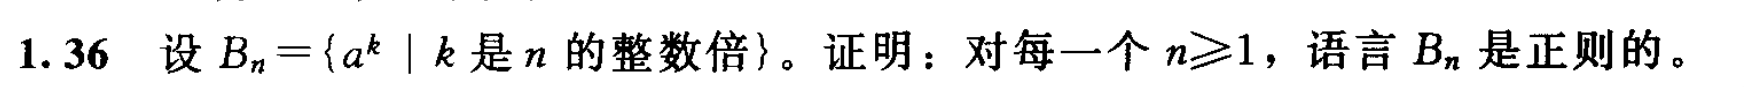
\includegraphics[width=\textwidth]{chapters/imgs/hw_1_36.png}
  \caption{}
  \label{fig:hw_1_36}
\end{figure}

\subsubsection*{证明}

固定任意 $n\ge 1$。构造 DFA
\[
    M_n=(Q,\{a\},\delta,q_0,F),
\]
其中
\[
    Q=\{q_0,q_1,\ldots,q_{n-1}\},\qquad F=\{q_0\}.
\]
状态 $q_i$ 表示目前已经读入的 $a$ 的个数模 $n$ 余 $i$。转移函数定义为
\[
    \delta(q_i,a)=q_{i+1 \bmod n},
    \qquad 0\le i\le n-1.
\]

于是对任意 $k\ge 0$，
\[
    \delta^*(q_0,a^k)=q_{k\bmod n}.
\]
因此
\[
    a^k\in L(M_n)
    \iff
    \delta^*(q_0,a^k)=q_0
    \iff
    k\equiv 0\pmod n.
\]
也就是说，
\[
    L(M_n)=\{a^k\mid k\text{ 是 }n\text{ 的整数倍}\}=B_n.
\]
所以对每个 $n\ge 1$，$B_n$ 都由一个有限状态自动机识别，故 $B_n$ 是正则语言。$\blacksquare$

\paragraph{解释.}
这里 DFA 需要记住的不是完整的长度 $k$，而只是 $k$ 除以 $n$ 的余数。余数只有
\[
    0,1,\ldots,n-1
\]
这 $n$ 种可能，因此可以用有限多个状态记录。每读入一个 $a$，余数加 $1$ 并对 $n$ 取模；最终回到余数 $0$ 的状态，正好表示长度是 $n$ 的整数倍。

\subsection*{1.40}

\begin{figure}[H]
  \centering
  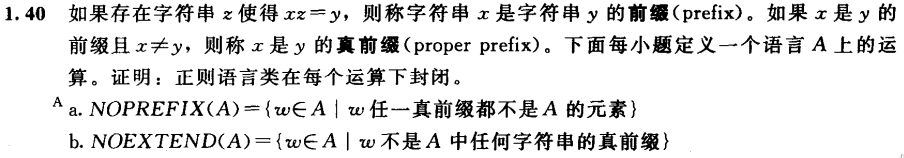
\includegraphics[width=\textwidth]{chapters/imgs/hw_1_40.png}
  \caption{}
  \label{fig:hw_1_40}
\end{figure}

\subsubsection*{证明}

设 $A$ 是正则语言，令
\[
    M=(Q,\Sigma,\delta,q_0,F)
\]
为识别 $A$ 的 DFA。

\begin{enumerate}[label=(\alph*), leftmargin=2.5em]
    \item 先证明 $\operatorname{NOPREFIX}(A)$ 正则。

    构造 DFA
    \[
        M_1=(Q\cup\{q_d\},\Sigma,\delta_1,q_0,F),
    \]
    其中 $q_d$ 是死状态。定义
    \[
        \delta_1(q_d,a)=q_d
        \qquad(a\in\Sigma),
    \]
    且对 $q\in Q$，
    \[
        \delta_1(q,a)=
        \begin{cases}
            q_d, & q\in F,\\
            \delta(q,a), & q\notin F.
        \end{cases}
    \]

    这个构造的含义是：一旦读到某个已经属于 $A$ 的前缀，而输入还没有结束，则该前缀就是真前缀，于是进入死状态。只有当第一次到达接受状态恰好发生在输入结束时，才接受。因此
    \[
        L(M_1)=\operatorname{NOPREFIX}(A),
    \]
    所以 $\operatorname{NOPREFIX}(A)$ 正则。

    \item 再证明 $\operatorname{NOEXTEND}(A)$ 正则。

    关键是筛掉那些“还能继续走到接受态”的状态。把 $M$ 看成一个有限有向图：状态是顶点，每条转移边
    \[
        q\xrightarrow{a}\delta(q,a)
    \]
    是一条带标号的有向边。定义
    \[
        P=\{q\in Q\mid \text{从 }q\text{ 出发存在一条长度至少为 }1\text{ 的路径通向 }F\}.
    \]
    等价地，
    \[
        P=\{q\in Q\mid \exists x\in\Sigma^+,\ \delta^*(q,x)\in F\}.
    \]
    这里并不是枚举无穷多个字符串 $x$，而是在有限状态图上做可达性判断。

    具体地，先在反向图中从所有接受状态 $F$ 出发做 BFS 或 DFS，得到
    \[
        R=\{q\in Q\mid \text{从 }q\text{ 出发可以经零步或多步到达 }F\}.
    \]
    然后取
    \[
        P=\{q\in Q\mid \exists a\in\Sigma,\ \delta(q,a)\in R\}.
    \]
    这样正好保证从 $q$ 到接受态至少走了一步；特别地，若某个接受状态有自环或能绕一圈回到接受状态，它也会被放入 $P$。

    构造 DFA
    \[
        M_2=(Q,\Sigma,\delta,q_0,F'),
        \qquad
        F'=F\setminus P.
    \]
    也就是说，状态、字母表、转移函数、开始状态全部不变，只把接受状态改为 $F\setminus P$。

    若 $w$ 被 $M_2$ 接受，设
    \[
        r=\delta^*(q_0,w).
    \]
    则 $r\in F'=F\setminus P$。所以 $r\in F$，从而 $w\in A$；同时 $r\notin P$，说明从 $r$ 出发不可能再经非空路径到达任何接受状态。于是不存在非空字符串 $z$ 使得 $wz\in A$，故 $w$ 不是 $A$ 中任何字符串的真前缀。

    反过来，若 $w\in A$ 且 $w$ 不是 $A$ 中任何字符串的真前缀，令 $r=\delta^*(q_0,w)$。由于 $w\in A$，有 $r\in F$；又因为 $w$ 不能继续扩展成 $A$ 中的字符串，从 $r$ 出发不存在通向接受状态的非空路径，所以 $r\notin P$。于是 $r\in F\setminus P=F'$，故 $M_2$ 接受 $w$。

    因此
    \[
        L(M_2)=\operatorname{NOEXTEND}(A),
    \]
    所以 $\operatorname{NOEXTEND}(A)$ 正则。
\end{enumerate}

综上，正则语言类在 $\operatorname{NOPREFIX}$ 与 $\operatorname{NOEXTEND}$ 运算下封闭。$\blacksquare$

\paragraph{解释.}
$\operatorname{NOPREFIX}(A)$ 要求“在接受当前串之前，不能已经接受过某个真前缀”，所以 DFA 只需在读入过程中检查是否提前进入过接受状态；若提前接受后还有输入，就进入死状态。

这里使用的 $\delta^*$ 是 DFA 转移函数 $\delta$ 的扩展。若
\[
    \delta:Q\times\Sigma\to Q
\]
表示读入一个字符后的状态转移，则
\[
    \delta^*:Q\times\Sigma^*\to Q
\]
表示从某个状态出发，读完整个字符串后到达的状态。它由
\[
    \delta^*(q,\varepsilon)=q,
    \qquad
    \delta^*(q,wa)=\delta(\delta^*(q,w),a)
\]
递归定义，其中 $w\in\Sigma^*$，$a\in\Sigma$。因此 $\delta^*(q,z)\in F$ 的意思是：从状态 $q$ 出发读完整个字符串 $z$ 后到达接受状态。这是自动机理论中的标准记号。

$\operatorname{NOEXTEND}(A)$ 要求“当前串虽然在 $A$ 中，但不能继续扩展成另一个 $A$ 中的串”。从改 DFA 的角度看，就是检查每个接受状态后面是否还存在通往某个接受状态的非空路径：若存在，就说明停在该状态的字符串还能继续扩展成 $A$ 中更长的字符串，因此这个状态不能保留为接受状态；若不存在，才保留它。这个过程完全发生在有限状态图上，所以是有限的构造。

\paragraph{什么叫封闭.}
一般地，称一类语言 $\mathcal C$ 在某个运算 $T$ 下封闭，是指对 $\mathcal C$ 中的语言施行该运算后，所得结果仍属于 $\mathcal C$。若 $T$ 是一元运算，则要求
\[
    A\in\mathcal C\implies T(A)\in\mathcal C;
\]
若 $T$ 是二元运算，则要求
\[
    A,B\in\mathcal C\implies T(A,B)\in\mathcal C.
\]
在本章里，$\mathcal C$ 就是正则语言类。因此 1.40 的结论是：若 $A$ 正则，则 $\operatorname{NOPREFIX}(A)$ 与 $\operatorname{NOEXTEND}(A)$ 仍正则。证明这类封闭性命题的常见方法，就是从识别原语言的 DFA 或 NFA 出发，直接构造识别新语言的自动机。

\subsection*{1.42}

\begin{figure}[H]
  \centering
  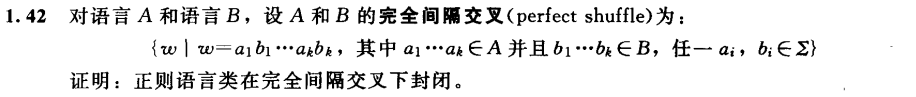
\includegraphics[width=\textwidth]{chapters/imgs/hw_1_42.png}
  \caption{}
  \label{fig:hw_1_42}
\end{figure}

\subsubsection*{证明}

设 $A,B\subseteq\Sigma^*$ 都是正则语言。取识别它们的 DFA
\[
    M_A=(Q_A,\Sigma,\delta_A,q_A,F_A),
    \qquad
    M_B=(Q_B,\Sigma,\delta_B,q_B,F_B).
\]
我们构造 DFA
\[
    M=(Q_A\times Q_B\times\{0,1\},\Sigma,\delta,(q_A,q_B,0),F),
\]
其中第三个分量用来记录当前读入的位置奇偶：
\[
    0:\text{下一位应送入 }M_A,
    \qquad
    1:\text{下一位应送入 }M_B.
\]
接受状态取为
\[
    F=F_A\times F_B\times\{0\}.
\]
这表示输入已经恰好读完若干对符号，并且奇数位形成的串被 $M_A$ 接受，偶数位形成的串被 $M_B$ 接受。

转移函数定义为
\[
    \delta\bigl((p,q,0),a\bigr)=(\delta_A(p,a),q,1),
    \qquad
    \delta\bigl((p,q,1),b\bigr)=(p,\delta_B(q,b),0),
\]
其中 $p\in Q_A$，$q\in Q_B$，$a,b\in\Sigma$。

下面证明 $L(M)$ 正是 $A$ 与 $B$ 的完全间隔交叉。

若
\[
    w=a_1b_1a_2b_2\cdots a_kb_k
\]
且
\[
    a_1a_2\cdots a_k\in A,\qquad b_1b_2\cdots b_k\in B,
\]
则 $M$ 读入奇数位时只更新第一个分量，读入偶数位时只更新第二个分量。因此读完整个 $w$ 后到达状态
\[
    \bigl(\delta_A^*(q_A,a_1a_2\cdots a_k),\ \delta_B^*(q_B,b_1b_2\cdots b_k),\ 0\bigr).
\]
由于两行分别属于 $A$ 与 $B$，前两个分量落在 $F_A$ 与 $F_B$ 中；又因为 $w$ 长度为偶数，第三个分量回到 $0$。故 $w\in L(M)$。

反过来，若 $w\in L(M)$，则第三个分量最终为 $0$，所以 $w$ 的长度必为偶数。于是可唯一写成
\[
    w=a_1b_1a_2b_2\cdots a_kb_k.
\]
设
\[
    x=a_1a_2\cdots a_k,
    \qquad
    y=b_1b_2\cdots b_k.
\]
根据转移定义，$M$ 读完 $w$ 后的前两个分量分别正是
\[
    \delta_A^*(q_A,x),
    \qquad
    \delta_B^*(q_B,y).
\]
又因为 $w$ 被接受，这两个状态分别属于 $F_A$ 与 $F_B$，故
\[
    x\in A,\qquad y\in B.
\]
因此 $w$ 正是由 $x\in A$ 与 $y\in B$ 按完全间隔交叉得到的字符串。

综上，
\[
    L(M)=\{w\mid w \text{ 是 }A\text{ 与 }B\text{ 的完全间隔交叉}\}.
\]
所以正则语言类在完全间隔交叉运算下封闭。$\blacksquare$

\paragraph{解释.}
这个构造的核心很直接：DFA 一边读输入，一边把奇数位送给识别 $A$ 的自动机，把偶数位送给识别 $B$ 的自动机；额外的一个二值状态只负责记录“当前该轮到哪一边读”。由于需要记住的信息只有两个分自动机的当前状态以及当前位置的奇偶性，所以总状态数仍然是有限的。

就 1.42 而言，这里讨论的运算是“完全间隔交叉”：输入是两个语言 $A,B$，输出是由 $A$ 中字符串与 $B$ 中字符串按奇偶位交错得到的所有字符串组成的语言。所谓“正则语言类在这个运算下封闭”，意思正是：只要 $A$ 与 $B$ 都正则，那么它们的完全间隔交叉所得语言也仍然正则。上面的乘积 DFA 就给出了这一点的构造性证明。

\subsection*{1.52}

\begin{figure}[H]
  \centering
  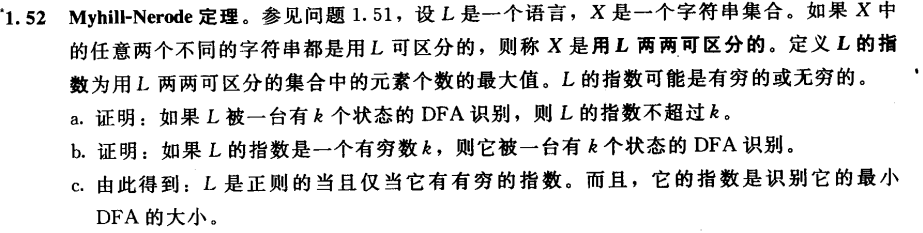
\includegraphics[width=\textwidth]{chapters/imgs/hw_1_52.png}
  \caption{}
  \label{fig:hw_1_52}
\end{figure}

\subsubsection*{证明}

记
\[
    x\equiv_L y
\]
表示字符串 $x,y\in\Sigma^*$ 用 $L$ 不可区分，即
\[
    \forall z\in\Sigma^*,\qquad xz\in L\iff yz\in L.
\]
若存在某个 $z\in\Sigma^*$ 使得
\[
    xz\in L,\ yz\notin L
\]
或反过来，则称 $x,y$ 可由 $L$ 区分。

\begin{enumerate}[label=(\alph*), leftmargin=2.5em]
    \item 设 $L$ 被一台有 $k$ 个状态的 DFA
    \[
        M=(Q,\Sigma,\delta,q_0,F)
    \]
    识别，并且 $|Q|=k$。任取一个用 $L$ 两两可区分的集合
    \[
        X\subseteq\Sigma^*.
    \]

    对每个 $x\in X$，看它从初态出发到达的状态 $\delta^*(q_0,x)$。若存在不同的 $x,y\in X$ 满足
    \[
        \delta^*(q_0,x)=\delta^*(q_0,y),
    \]
    则对任意 $z\in\Sigma^*$，都有
    \[
        \delta^*(q_0,xz)
        =
        \delta^*(\delta^*(q_0,x),z)
        =
        \delta^*(\delta^*(q_0,y),z)
        =
        \delta^*(q_0,yz).
    \]
    因而
    \[
        xz\in L\iff yz\in L.
    \]
    这说明 $x,y$ 用 $L$ 不可区分，与 $X$ 中任意两个不同字符串都应可区分矛盾。

    因此，$X$ 中不同字符串必须到达不同状态。于是映射
    \[
        x\longmapsto \delta^*(q_0,x)
    \]
    从 $X$ 到 $Q$ 是单射，所以
    \[
        |X|\le |Q|=k.
    \]
    故 $L$ 的指数不超过 $k$。

    \item 设 $L$ 的指数有限，且等于 $k$。因为 $L$ 的指数为 $k$，所以关系 $\equiv_L$ 将 $\Sigma^*$ 分成 $k$ 个等价类。以这些等价类为状态，构造 DFA
    \[
        M=(Q,\Sigma,\delta,q_0,F).
    \]
    令
    \[
        Q=\{[x]\mid x\in\Sigma^*\},
    \]
    其中
    \[
        [x]=\{y\in\Sigma^*\mid y\equiv_L x\}.
    \]
    因为指数是 $k$，所以 $|Q|=k$。

    初始状态定义为
    \[
        q_0=[\varepsilon].
    \]

    转移函数定义为
    \[
        \delta([x],a)=[xa].
    \]
    需要说明它是良定义的。若
    \[
        [x]=[y],
    \]
    即 $x\equiv_L y$，则对任意 $z\in\Sigma^*$，因为 $x\equiv_L y$ 对字符串 $az$ 也成立，所以
    \[
        xaz\in L\iff yaz\in L.
    \]
    也就是
    \[
        (xa)z\in L\iff (ya)z\in L.
    \]
    因此 $xa\equiv_L ya$，从而
    \[
        [xa]=[ya].
    \]
    所以转移函数定义良好。

    接受状态定义为
    \[
        F=\{[x]\mid x\in L\}.
    \]
    这同样是良定义的。若 $[x]=[y]$，即 $x\equiv_L y$，取 $z=\varepsilon$，则
    \[
        x\in L\iff y\in L.
    \]
    因而同一个等价类中的字符串要么全在 $L$ 中，要么全不在 $L$ 中，所以接受状态集合定义良好。

    下面证明该 DFA 识别 $L$。对任意字符串
    \[
        w=a_1a_2\cdots a_n,
    \]
    由转移定义可归纳得到
    \[
        \delta^*([\varepsilon],w)=[w].
    \]
    因此
    \[
        w\in L(M)
        \iff
        \delta^*([\varepsilon],w)\in F
        \iff
        [w]\in F
        \iff
        w\in L.
    \]
    所以
    \[
        L(M)=L.
    \]
    因而 $L$ 被一台有 $k$ 个状态的 DFA 识别。

    \item 由 (a) 可知，若 $L$ 被某台 $k$ 状态 DFA 识别，则 $L$ 的指数不超过 $k$。因此，若 $L$ 是正则语言，则存在有限状态 DFA 识别它，从而 $L$ 的指数有限。

    由 (b) 可知，若 $L$ 的指数有限且等于 $k$，则可构造一台有 $k$ 个状态的 DFA 识别 $L$。所以
    \[
        L\text{ 正则}
        \iff
        L\text{ 的指数有限}.
    \]
    此外，因为任何识别 $L$ 的 DFA 的状态数都至少是 $L$ 的指数，而我们又能构造一台恰有指数个状态的 DFA，所以
    \[
        \boxed{
            L\text{ 的指数}
            =
            \text{识别 }L\text{ 的最小 DFA 的状态数}.
        }
    \]
    $\blacksquare$
\end{enumerate}

\paragraph{解释.}
Myhill--Nerode 定理的核心是：DFA 的一个状态只代表“从这里继续往后读，未来会发生什么”。若两个前缀 $x,y$ 对所有后缀 $z$ 都表现完全一样，即
\[
    xz\in L\iff yz\in L,
\]
那么自动机没有必要把它们分开；反之，只要存在某个后缀能把它们区分开，自动机就必须给它们不同的状态。因此，最小 DFA 的状态本质上就是这些“未来行为”不同的等价类。

\subsection*{1.53}

\begin{figure}[h]
  \centering
  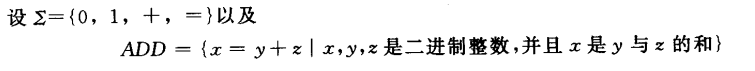
\includegraphics[width=\textwidth]{chapters/imgs/hw_1_53.png}
  \caption{}
  \label{fig:hw_1_53}
\end{figure}

\subsubsection*{证明}

设
\[
    \mathrm{ADD}
    =
    \{x=y+z\mid x,y,z\text{ 是二进制整数，且 }x=y+z\}.
\]
我们用闭包性质反证。令
\[
    R=\{10^i=10^j+0\mid i,j\ge 0\}.
\]
显然 $R$ 是正则语言，因为它可由正则表达式
\[
    10^*=10^*+0
\]
描述。

若 $\mathrm{ADD}$ 是正则语言，则
\[
    L=\mathrm{ADD}\cap R
\]
也应是正则语言。但在 $R$ 中，字符串具有形式
\[
    10^i=10^j+0.
\]
其表示的等式为
\[
    2^i=2^j+0.
\]
该等式成立当且仅当 $i=j$。因此
\[
    L=\{10^n=10^n+0\mid n\ge 0\}.
\]

下面证明 $L$ 非正则。假设 $L$ 正则，令 $p$ 为其泵长度。取
\[
    s=10^p=10^p+0\in L.
\]
由泵引理，存在分解 $s=xyz$，满足
\[
    |xy|\le p,\qquad |y|>0,
\]
且对所有 $k\ge 0$，都有 $xy^kz\in L$。

由于 $|xy|\le p$，子串 $y$ 完全落在第一个 $10^p$ 中。令 $k=0$，即删除 $y$。这样得到的 $xz$ 会改变等号左边的二进制数，而等号右边的 $10^p+0$ 不变。因此 $xz$ 不可能仍具有形式
\[
    10^n=10^n+0.
\]
所以
\[
    xz\notin L,
\]
这与泵引理矛盾。故 $L$ 非正则。

于是若 $\mathrm{ADD}$ 正则，则正则语言 $R$ 与它的交 $L$ 应正则；但 $L$ 非正则，矛盾。因此
\[
    \mathrm{ADD}
\]
不是正则语言。$\blacksquare$

\paragraph{解释.}
这个证明的关键是用正则语言 $R$ 把 $\mathrm{ADD}$ 限制到一种很简单的加法：
\[
    10^i=10^j+0.
\]
此时加法本身没有复杂性，因为右边只是加 $0$；唯一要检查的是左右两个二进制数是否完全相同，即是否 $i=j$。这就把问题化为
\[
    \{10^n=10^n+0\mid n\ge 0\},
\]
而有限自动机无法记住等号左边有多少个 $0$，再在等号右边逐一比较。因此该语言非正则，从而 $\mathrm{ADD}$ 也不可能正则。

\clearpage
